\appendix

\section{Effect of sampling duration on consistency of offline analysis of data}
\label{app:effectOfSamplingDuration}

Different grids can have their own set of `events', such as firing up of boilers or other kinds of switching events, or `cycles' of changes, such as sub-hourly power dispatches, semi-diurnal variation in solar generation, hourly wind power fluctuations, etc. A question then arises: Can the `statistical nature' of a grid be really generalized if it itself doesn't show a constant characteristic in its dynamics? The answer is: Yes, but only if a `sufficient' duration of data has been collected for analysis, such that all kinds of cyclical variations are `averaged-out' over the duration, displaying a somewhat consistent statistical signature irrespective of the actual time the analysis was made or data collected from.

Data for different years or months of select grids (Great Britain, France RTE, Nordic, Japan) mentioned in Table \ref{tab:realGridSamplingData} were compared in terms of their Fixed Time Autocorrelation plots (Autocorrelation Decay Curves). The plots were a mixture of year-wise (Nordic), month-wise (Great Britain, France RTE, Tokyo) and day-wise (Indian NRLDC) data. It was concluded that, barring some small vertical shifts among the autocorrelation values, the trends were consistently displayed for year-wise and month-wise plots, but did not show consistency in their day-to-day plots. 

\begin{figure}[!ht]
	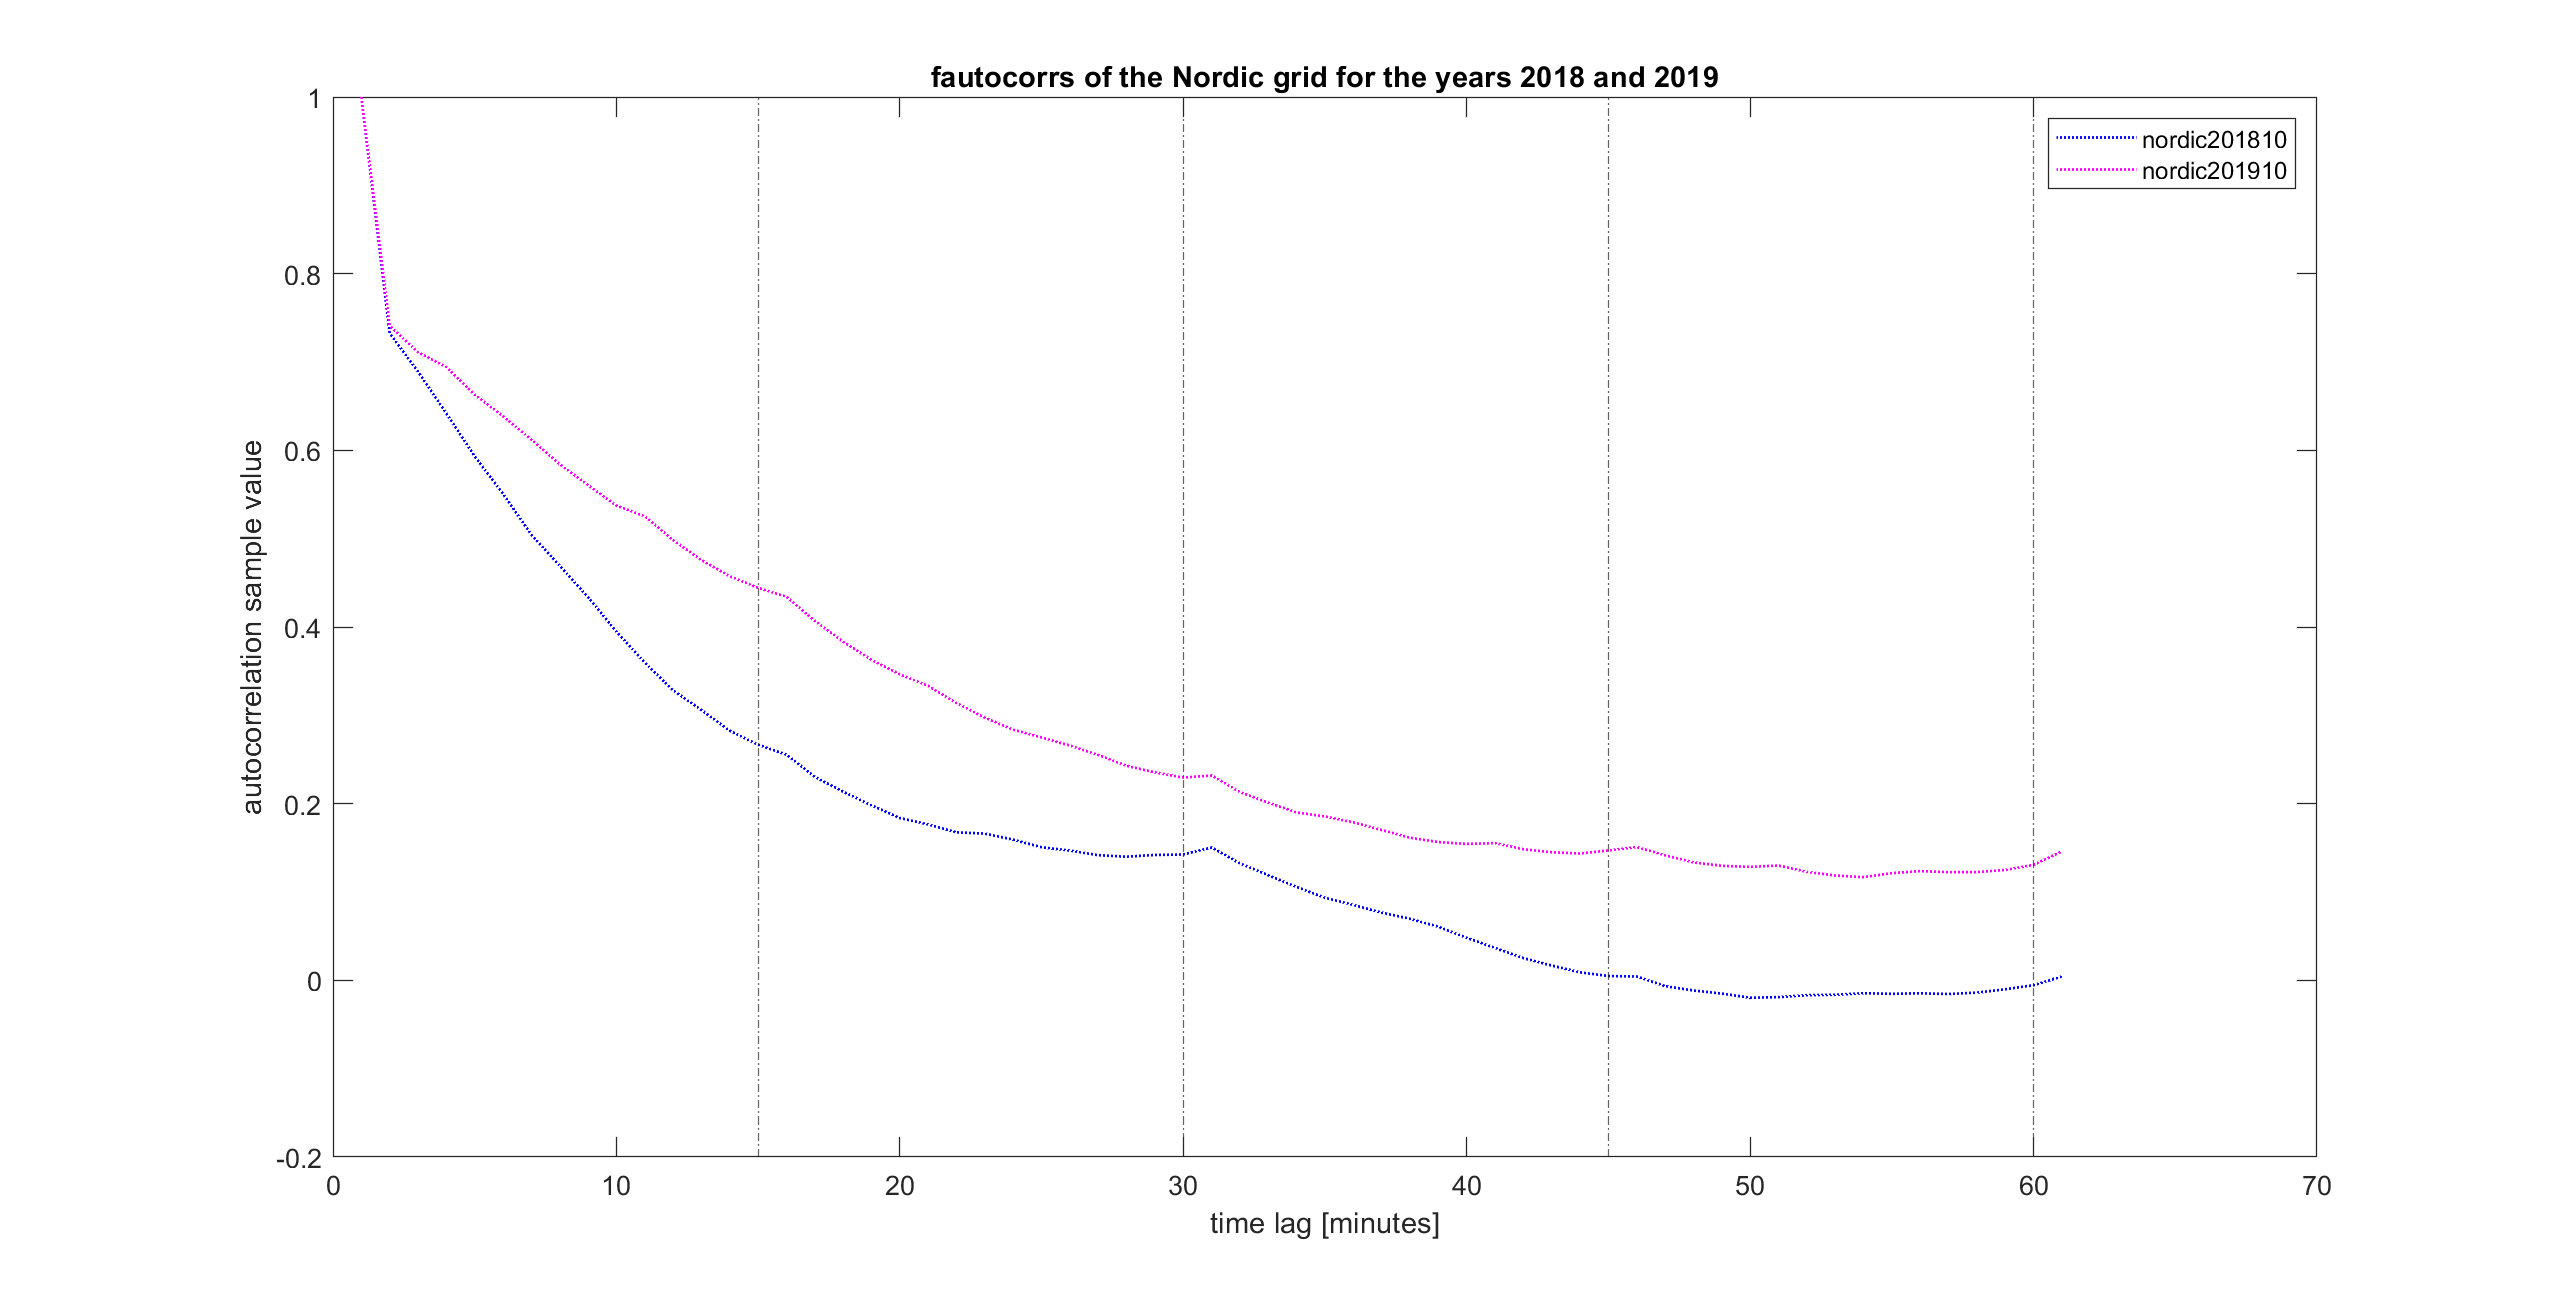
\includegraphics[scale=0.25]{../figures/autocorr/fautocorrs_nordic_201801_to_201912}
	\caption{Fixed Time Autocorrelation plots for the Nordic Grid for two consecutive years, 2018 and 2019. They present a fairly consistent picture of the grid's dynamics, with only a minor difference in the magnitude of the autocorrelation values.}
\end{figure}


\begin{figure}[!ht]
	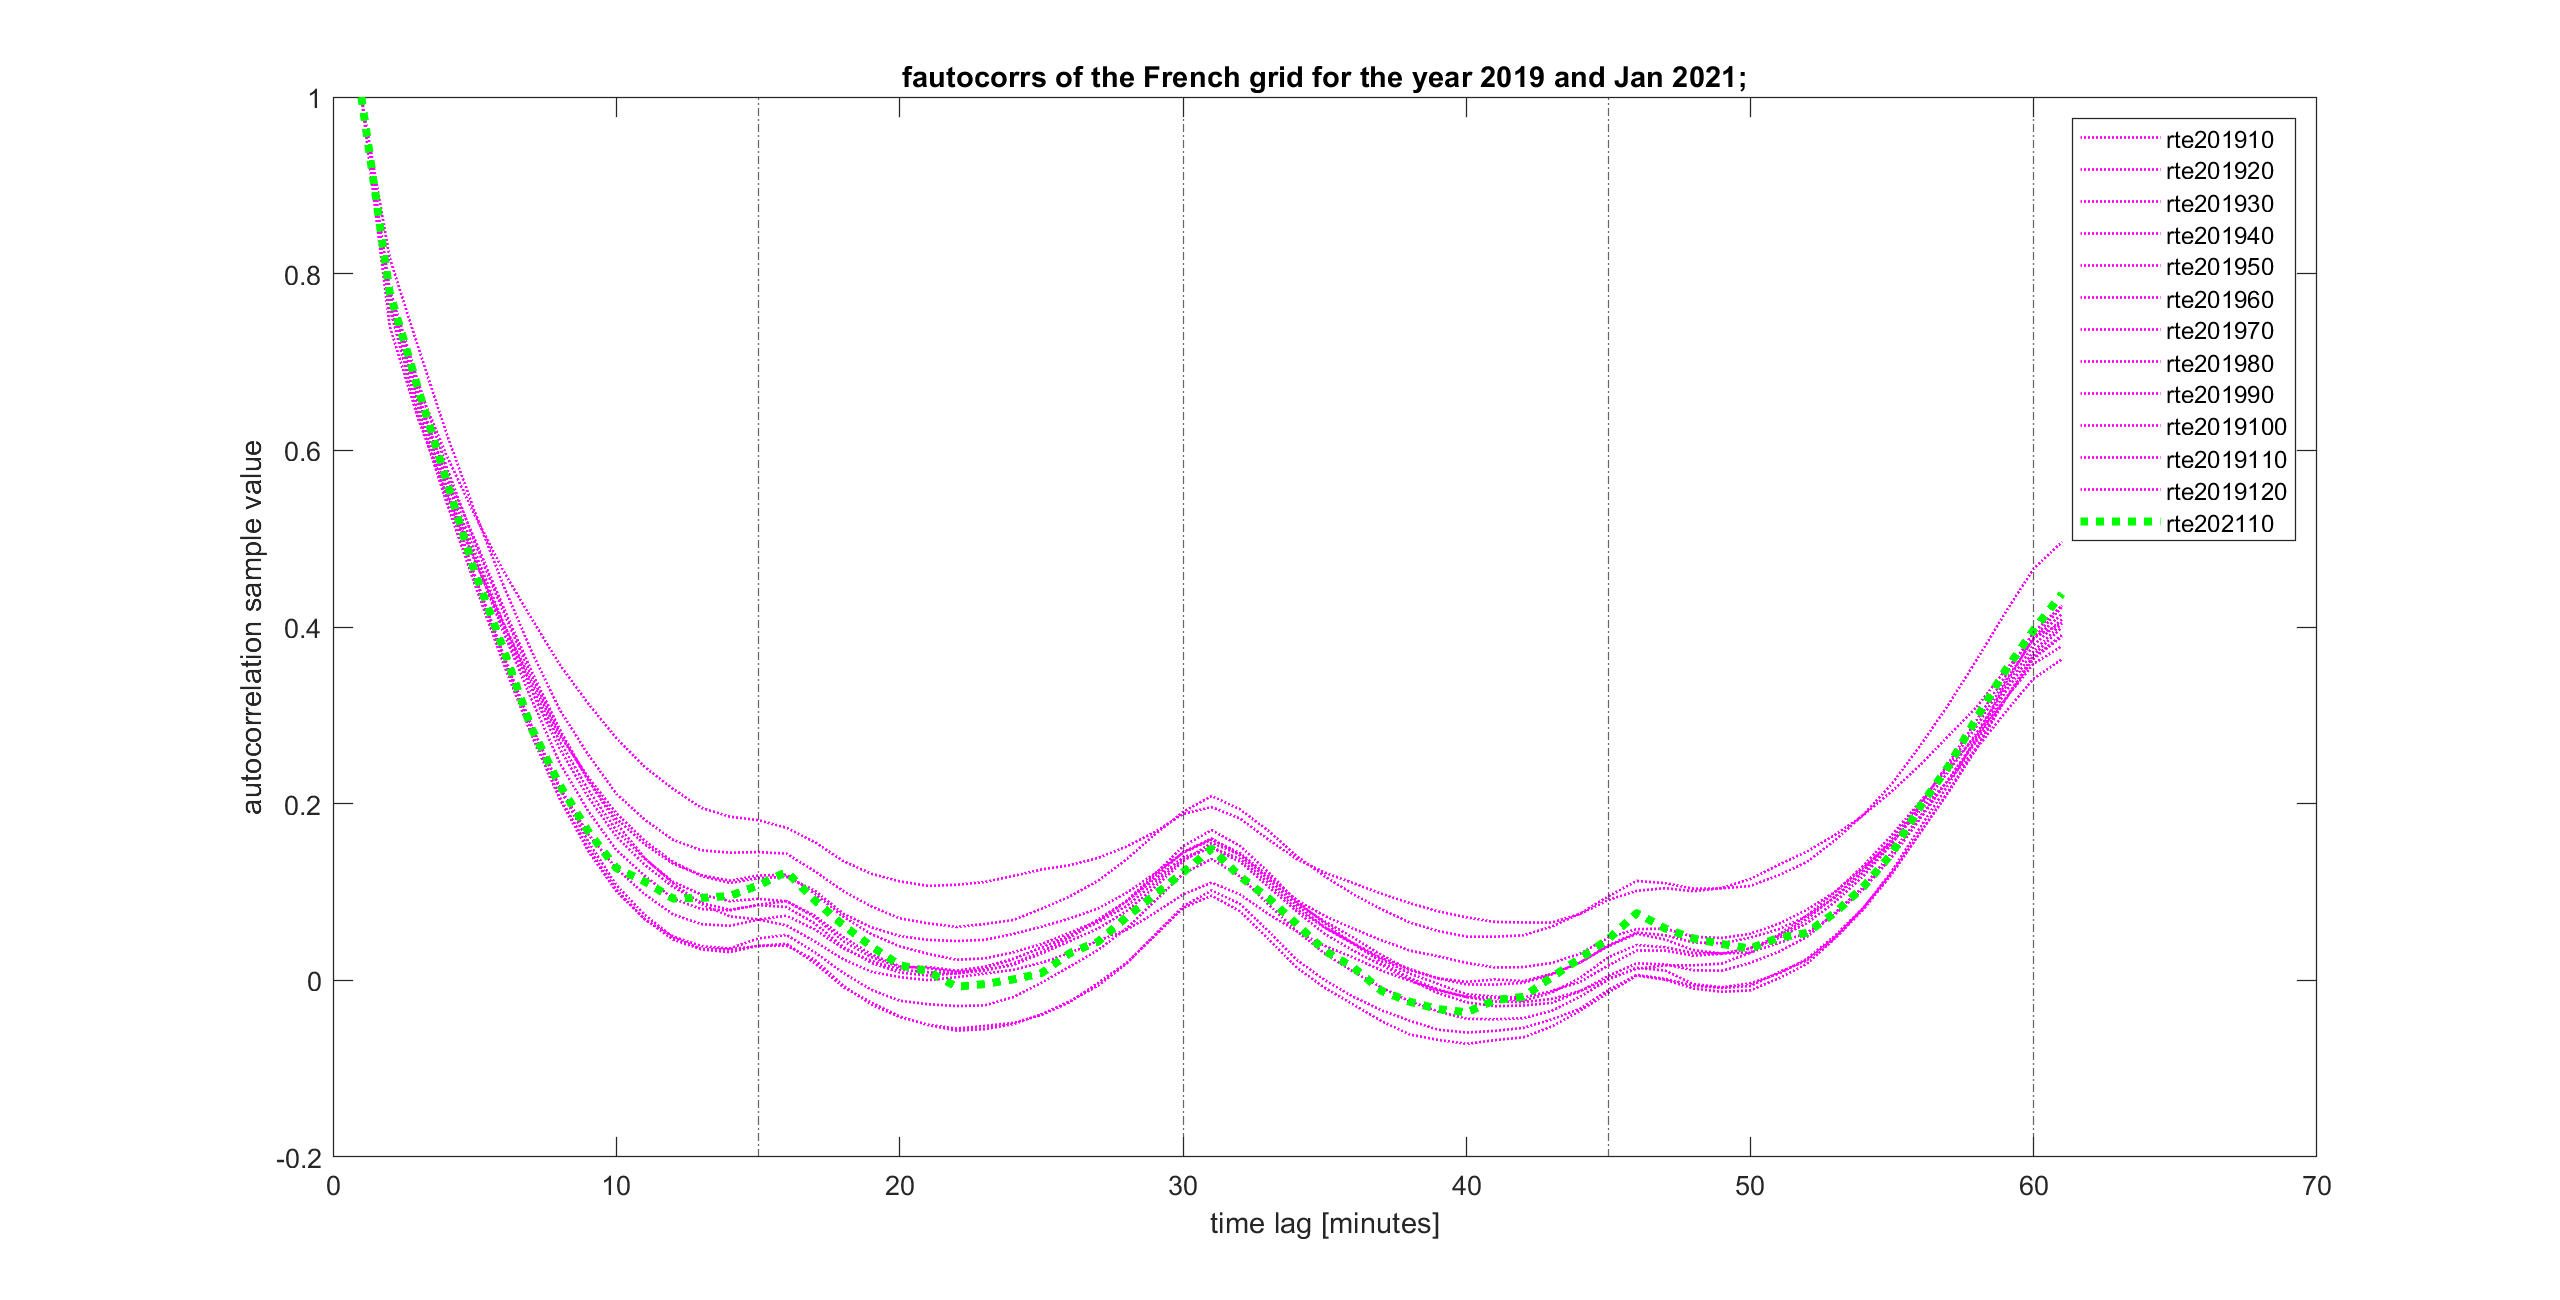
\includegraphics[scale=0.25]{../figures/autocorr/fautocorrs_rte_201901_to_201912_202101}
		\caption{Fixed Time Autocorrelation plots for the French Grid for twelve months of the year 2019 and January 2021. They present a fairly consistent picture of the grid's dynamics.}
\end{figure}

\begin{figure}[!ht]
	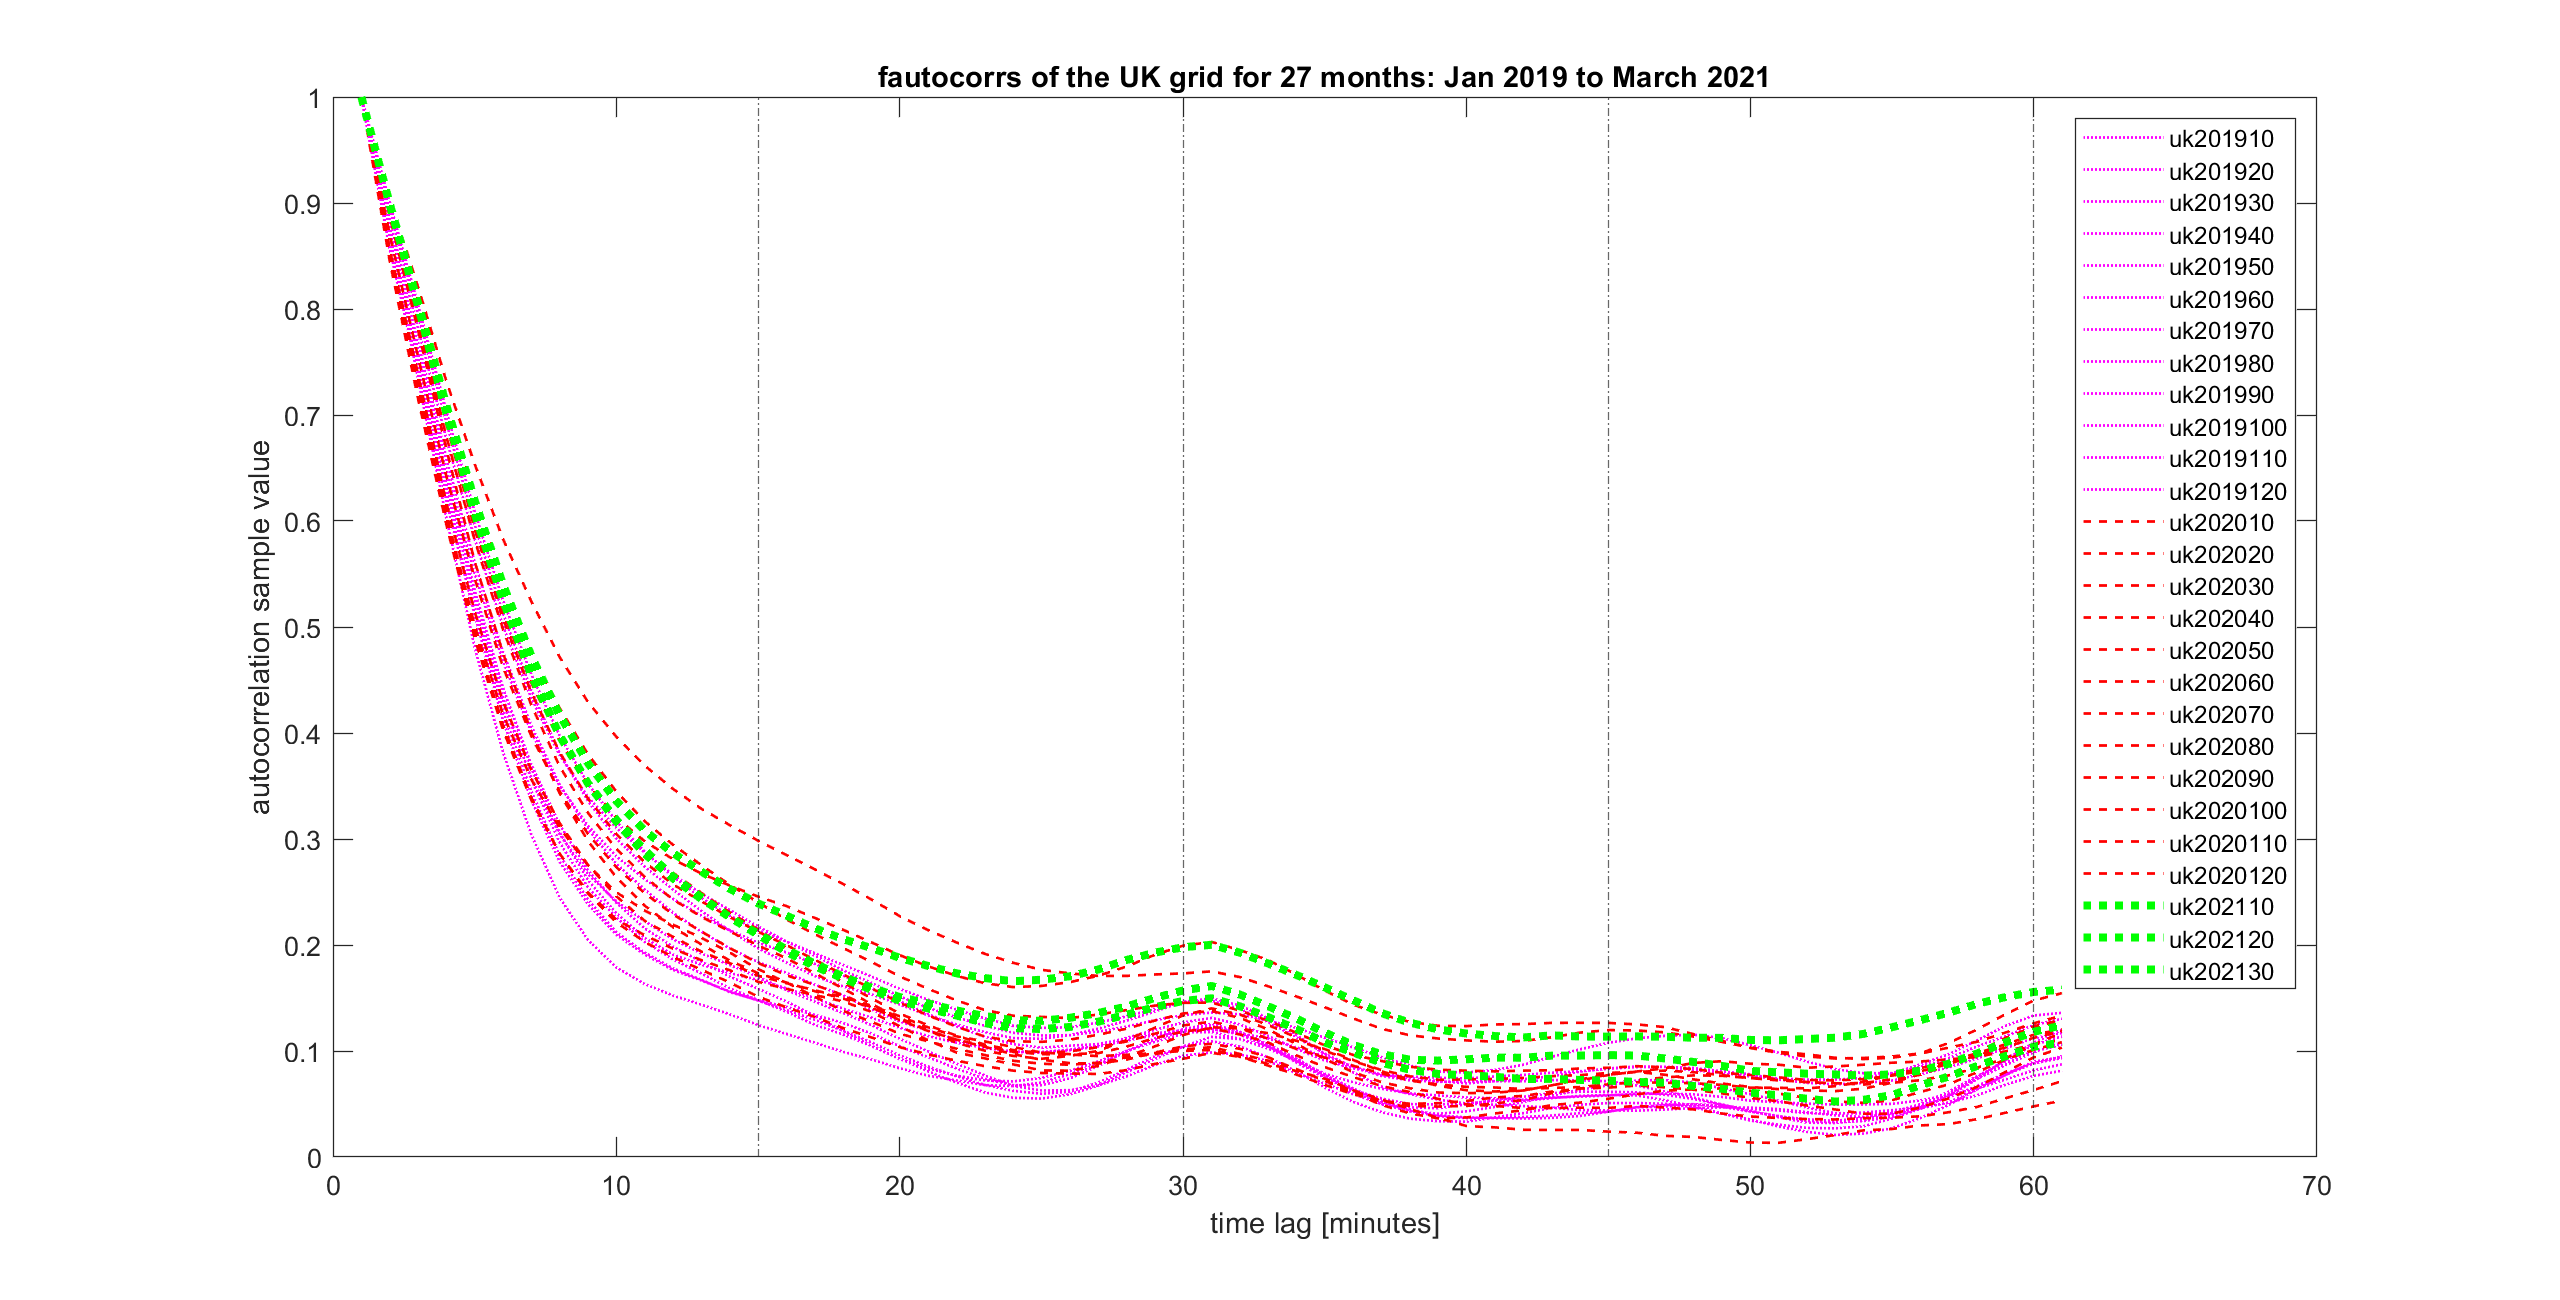
\includegraphics[scale=0.25]{../figures/autocorr/fautocorrs_uk_201901_to_202103_2}
	\caption{Fixed Time Autocorrelation plots for the Great Britain Grid for twenty seven continuous months, from January 2019 to March 2021. They present a fairly consistent picture of the grid's dynamics.}
\end{figure}

\begin{figure}[!ht]
	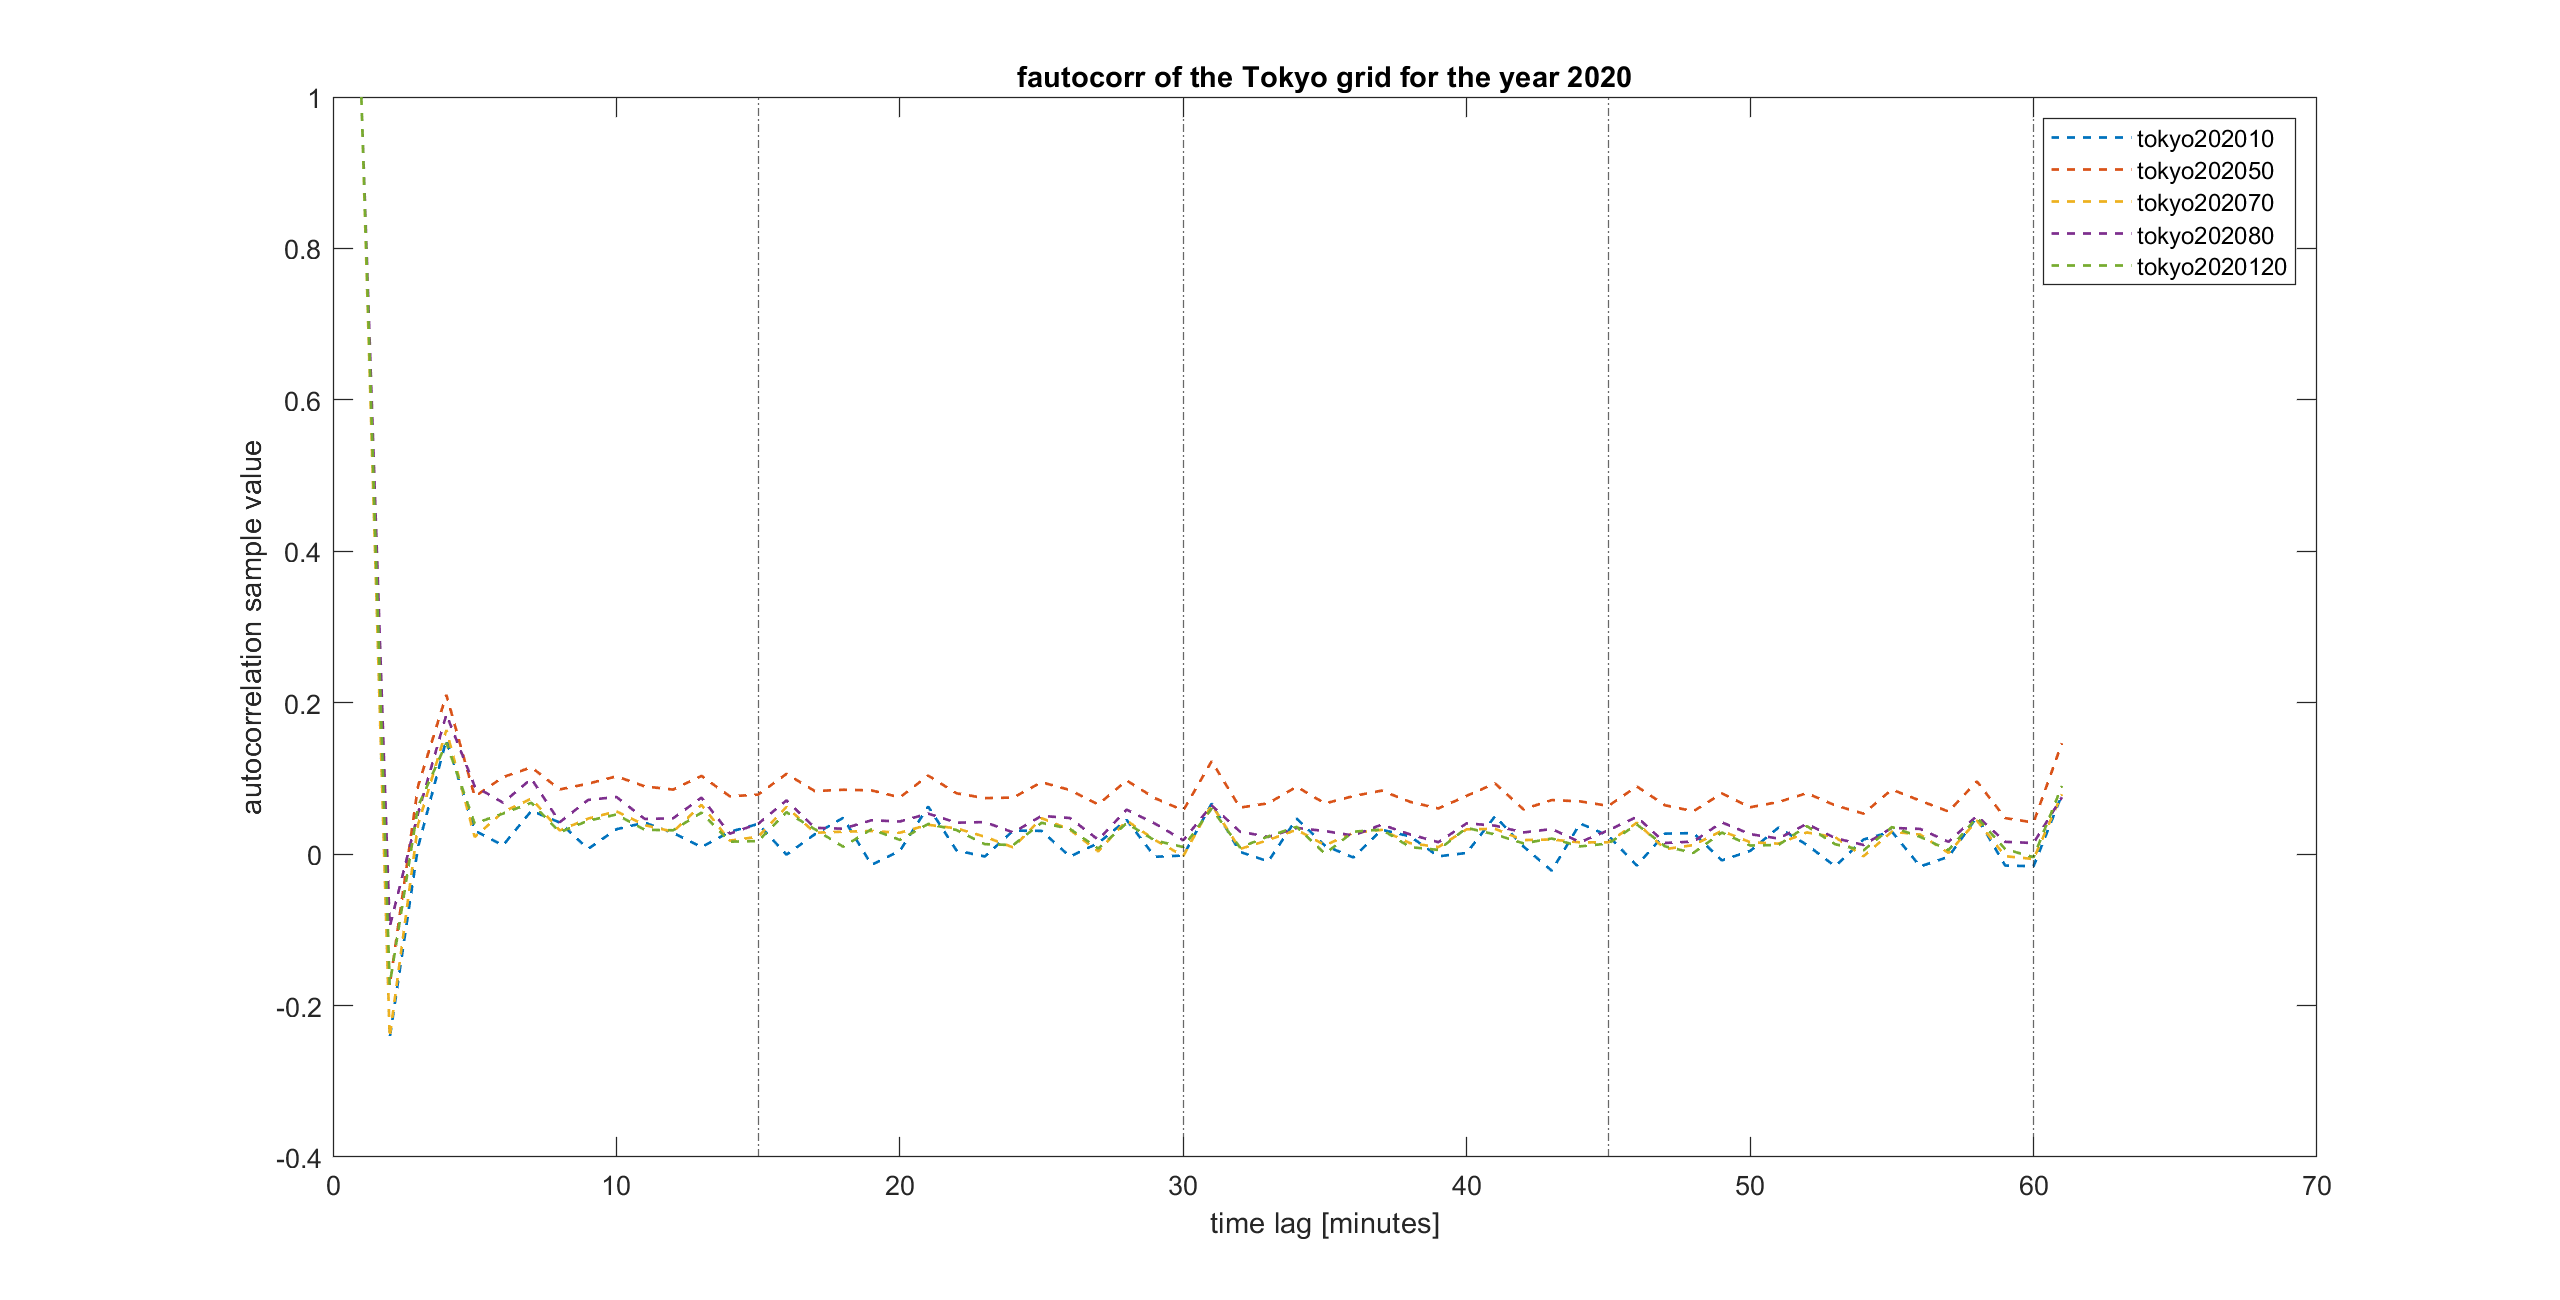
\includegraphics[scale=0.25]{../figures/autocorr/fautocorrs_tokyo_202001_to_202012}
	\caption{Fixed Time Autocorrelation plots for the Tokyo Grid for five non-continuous months of the year 2020: January, May, July, August and December. They present a fairly consistent picture of the grid's dynamics.}
\end{figure}

Data for six non-continuous days (07 April 2019, 03 July 2019, 08 August 2019, 14 December 2019, 01 February 2020 and 05 April 2020) for the Indian grid (NRLDC) was also compared in a similar fashion. Some of the days have also been marked with attributes to indicate notable demand-generation characteristics associated with the day, including: Day with minimum renewable generation, Day with maximum renewable generation contribution (07 April 2019), Day with minimum solar power contribution (08 August 2019), Day with lowest power demand (14 December 2019) and Day with lowest renewable generation contribution (01 February 2020). The plots were inconsistent and therefore a day's worth of data could be considered insufficient to average-out all the dynamic differences in a grid's statistical signature.

\begin{figure}[!ht]
	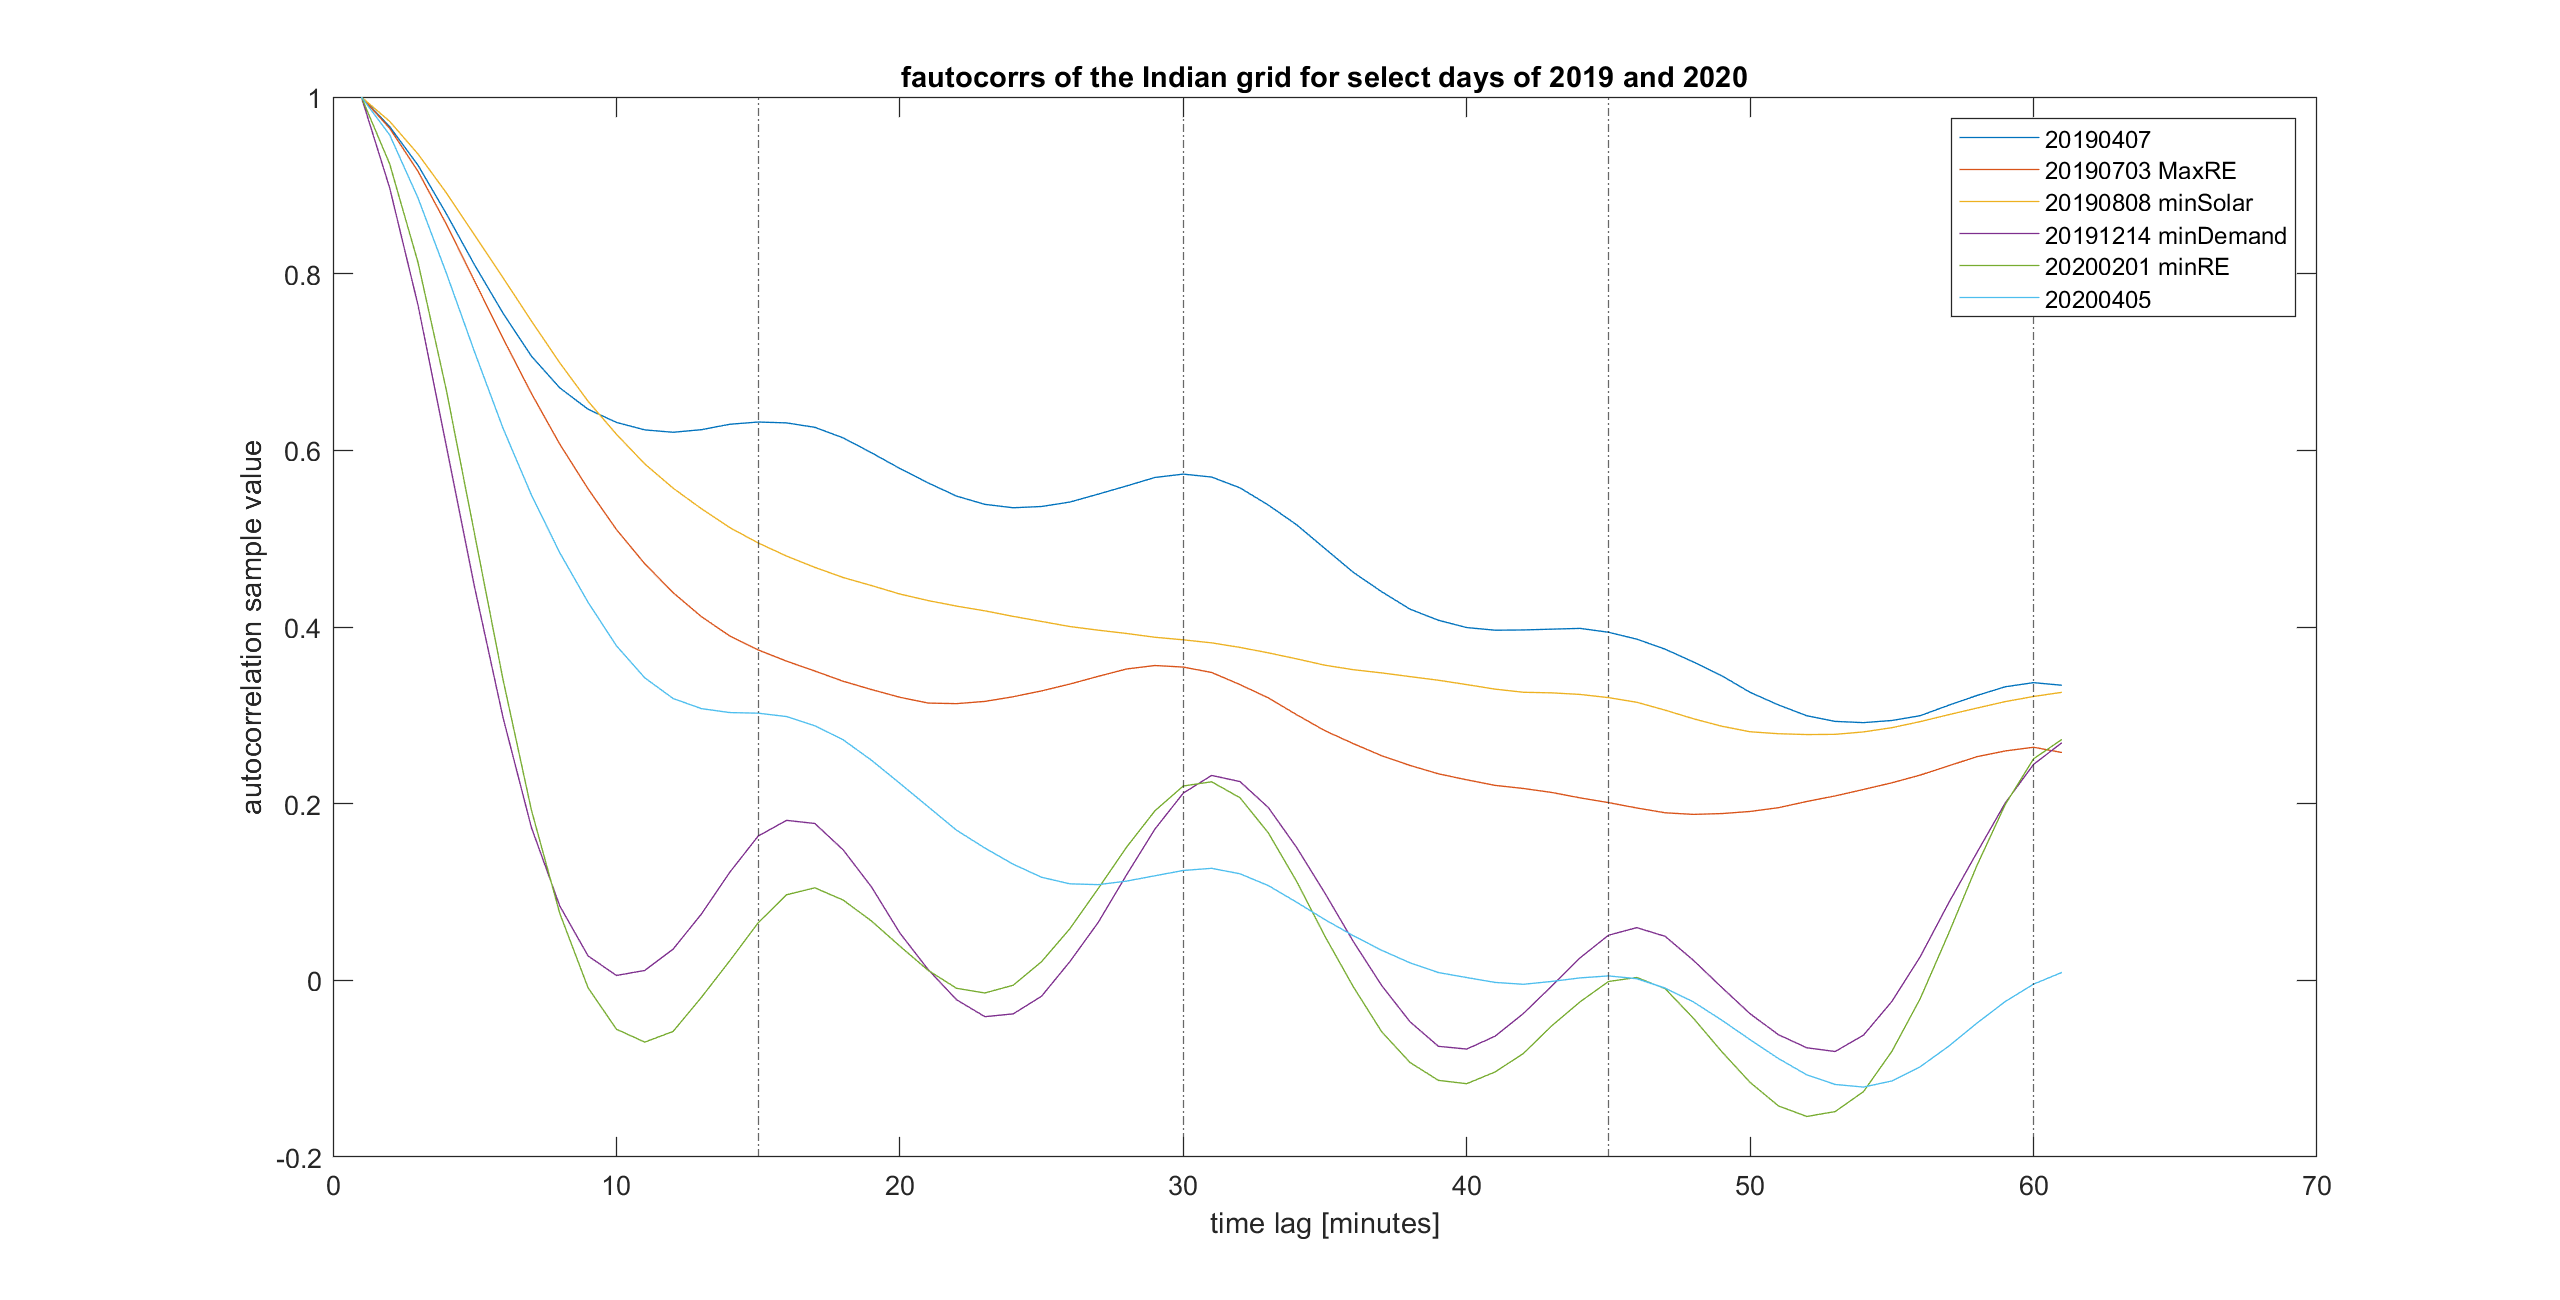
\includegraphics[scale=0.25]{../figures/autocorr/fautocorrs_nrldc_201904_to_202004}
	\caption{Fixed Time Autocorrelation Plots for Six non-continuous days of the Indian Grid: 07 April 2019, 03 July 2019, 08 August 2019, 14 December 2019, 01 February 2020 and 05 April 2020. Some of the days have also been marked with attributes with notable demand-generation characteristics associated with the day.}
\end{figure}

\begin{figure}[htp]
	\centering
	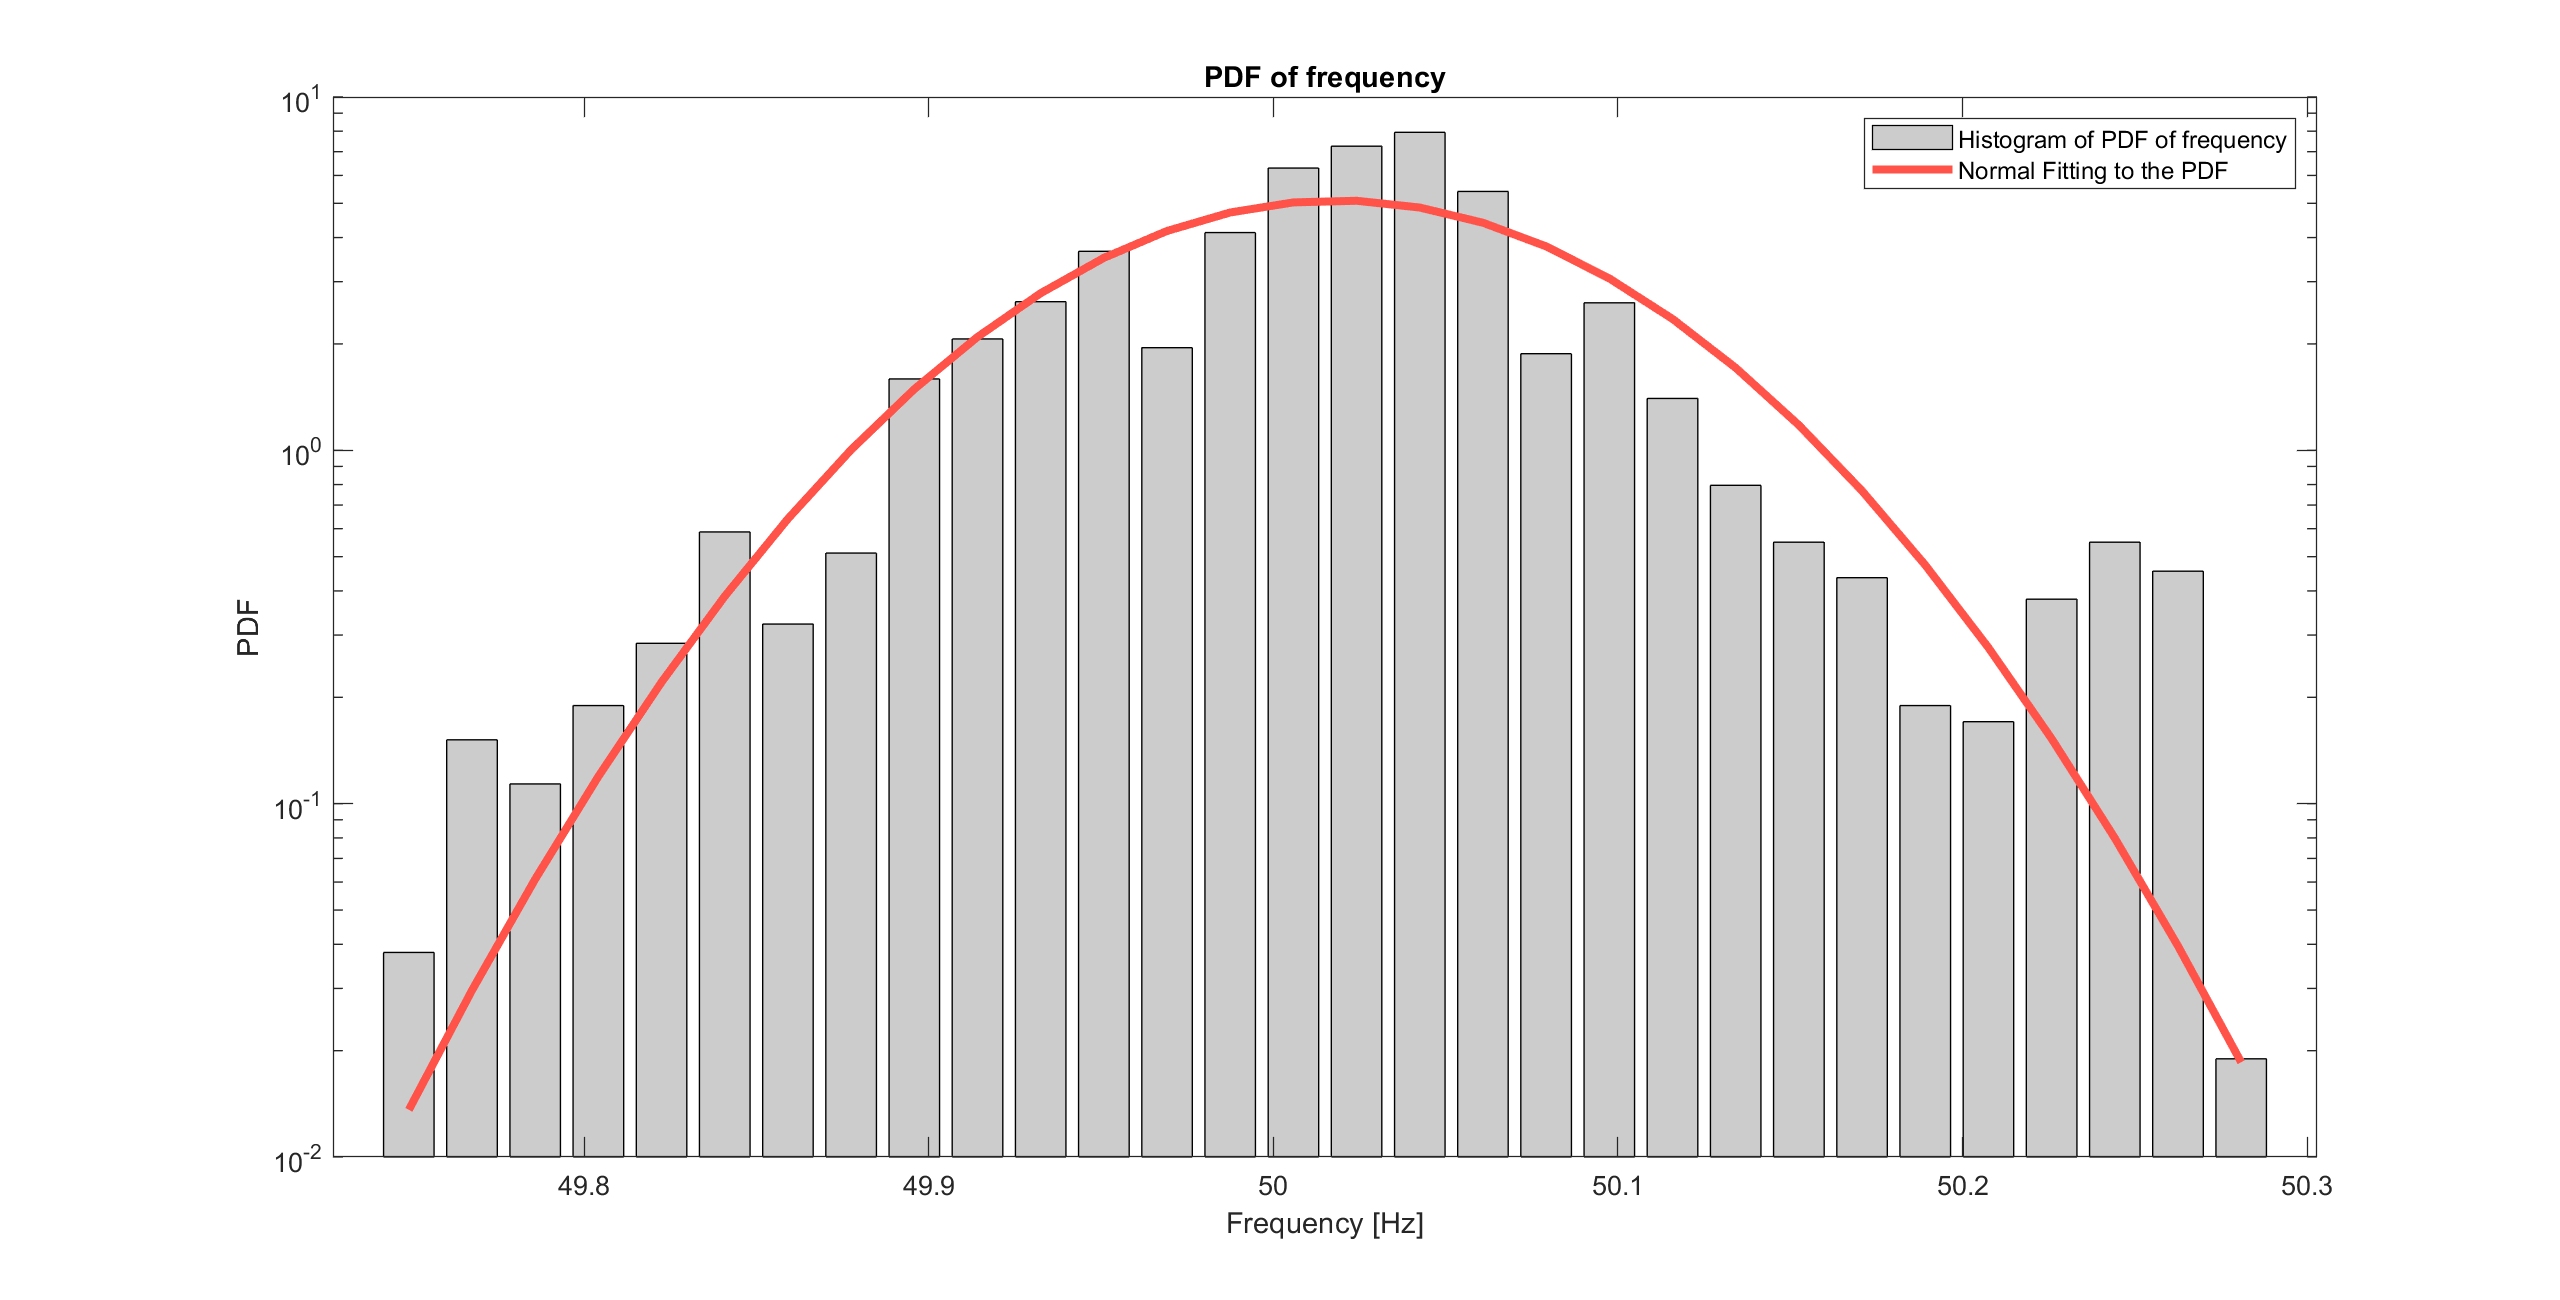
\includegraphics[width=.45\textwidth]{../figures/pdf/nrldc/pdf_frequency_nrldc_01}\quad
	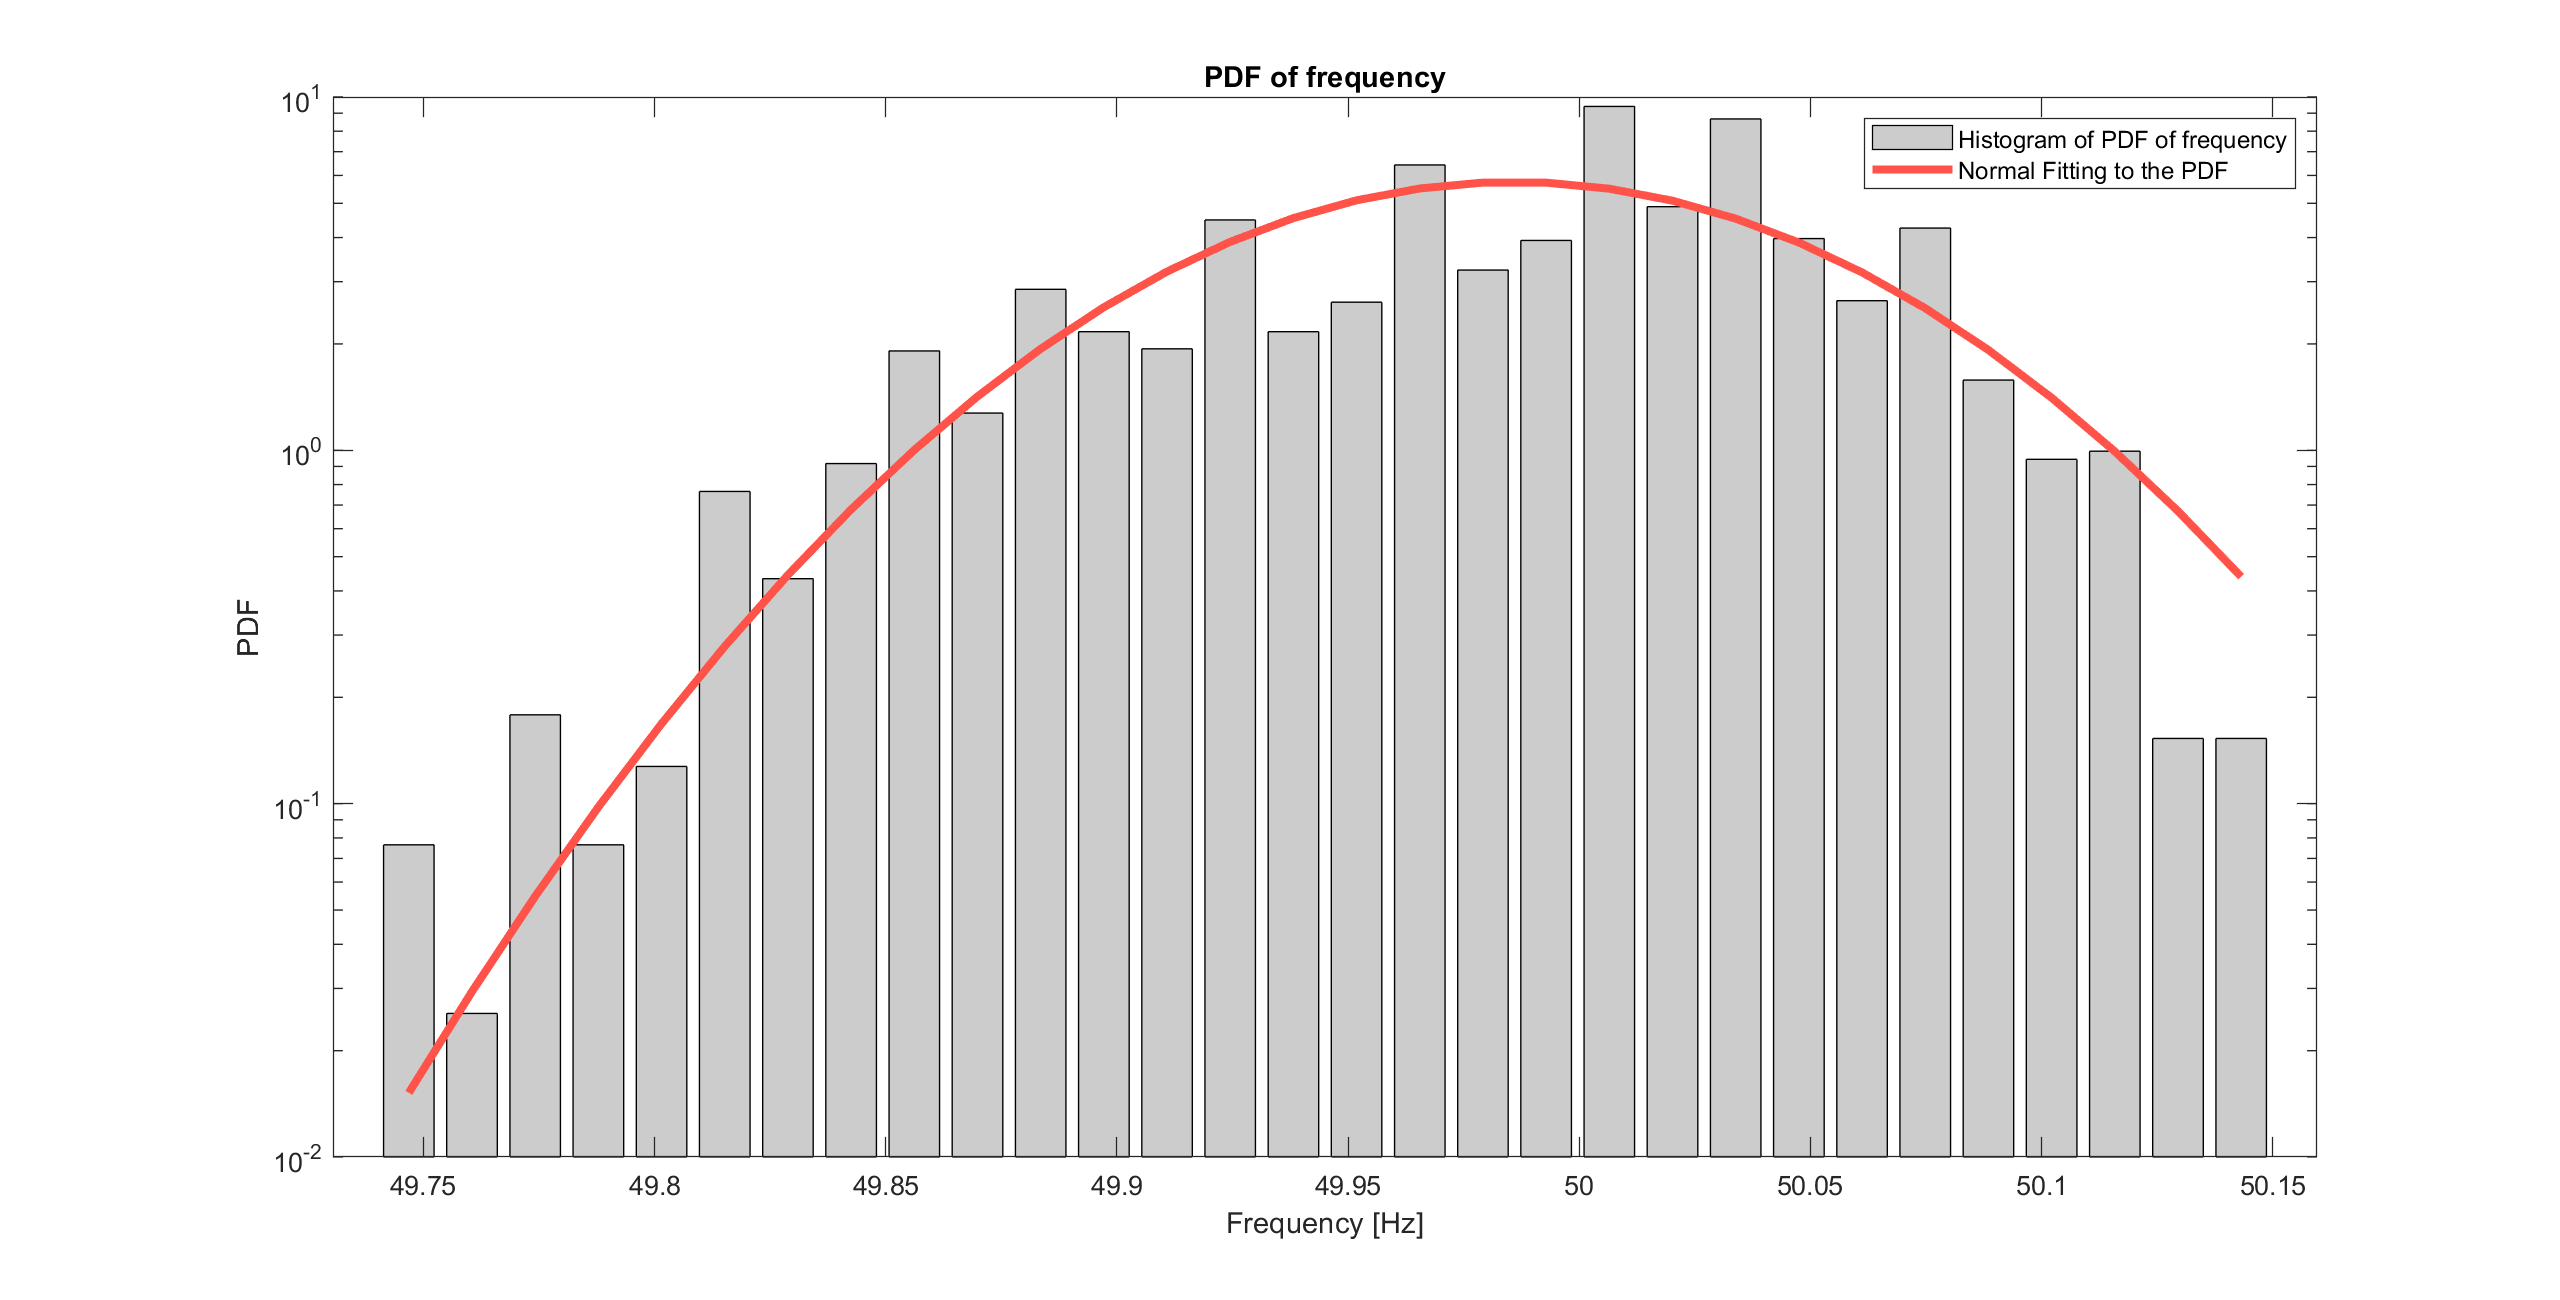
\includegraphics[width=.45\textwidth]{../figures/pdf/nrldc/pdf_frequency_nrldc_02}
	
	\medskip
	
	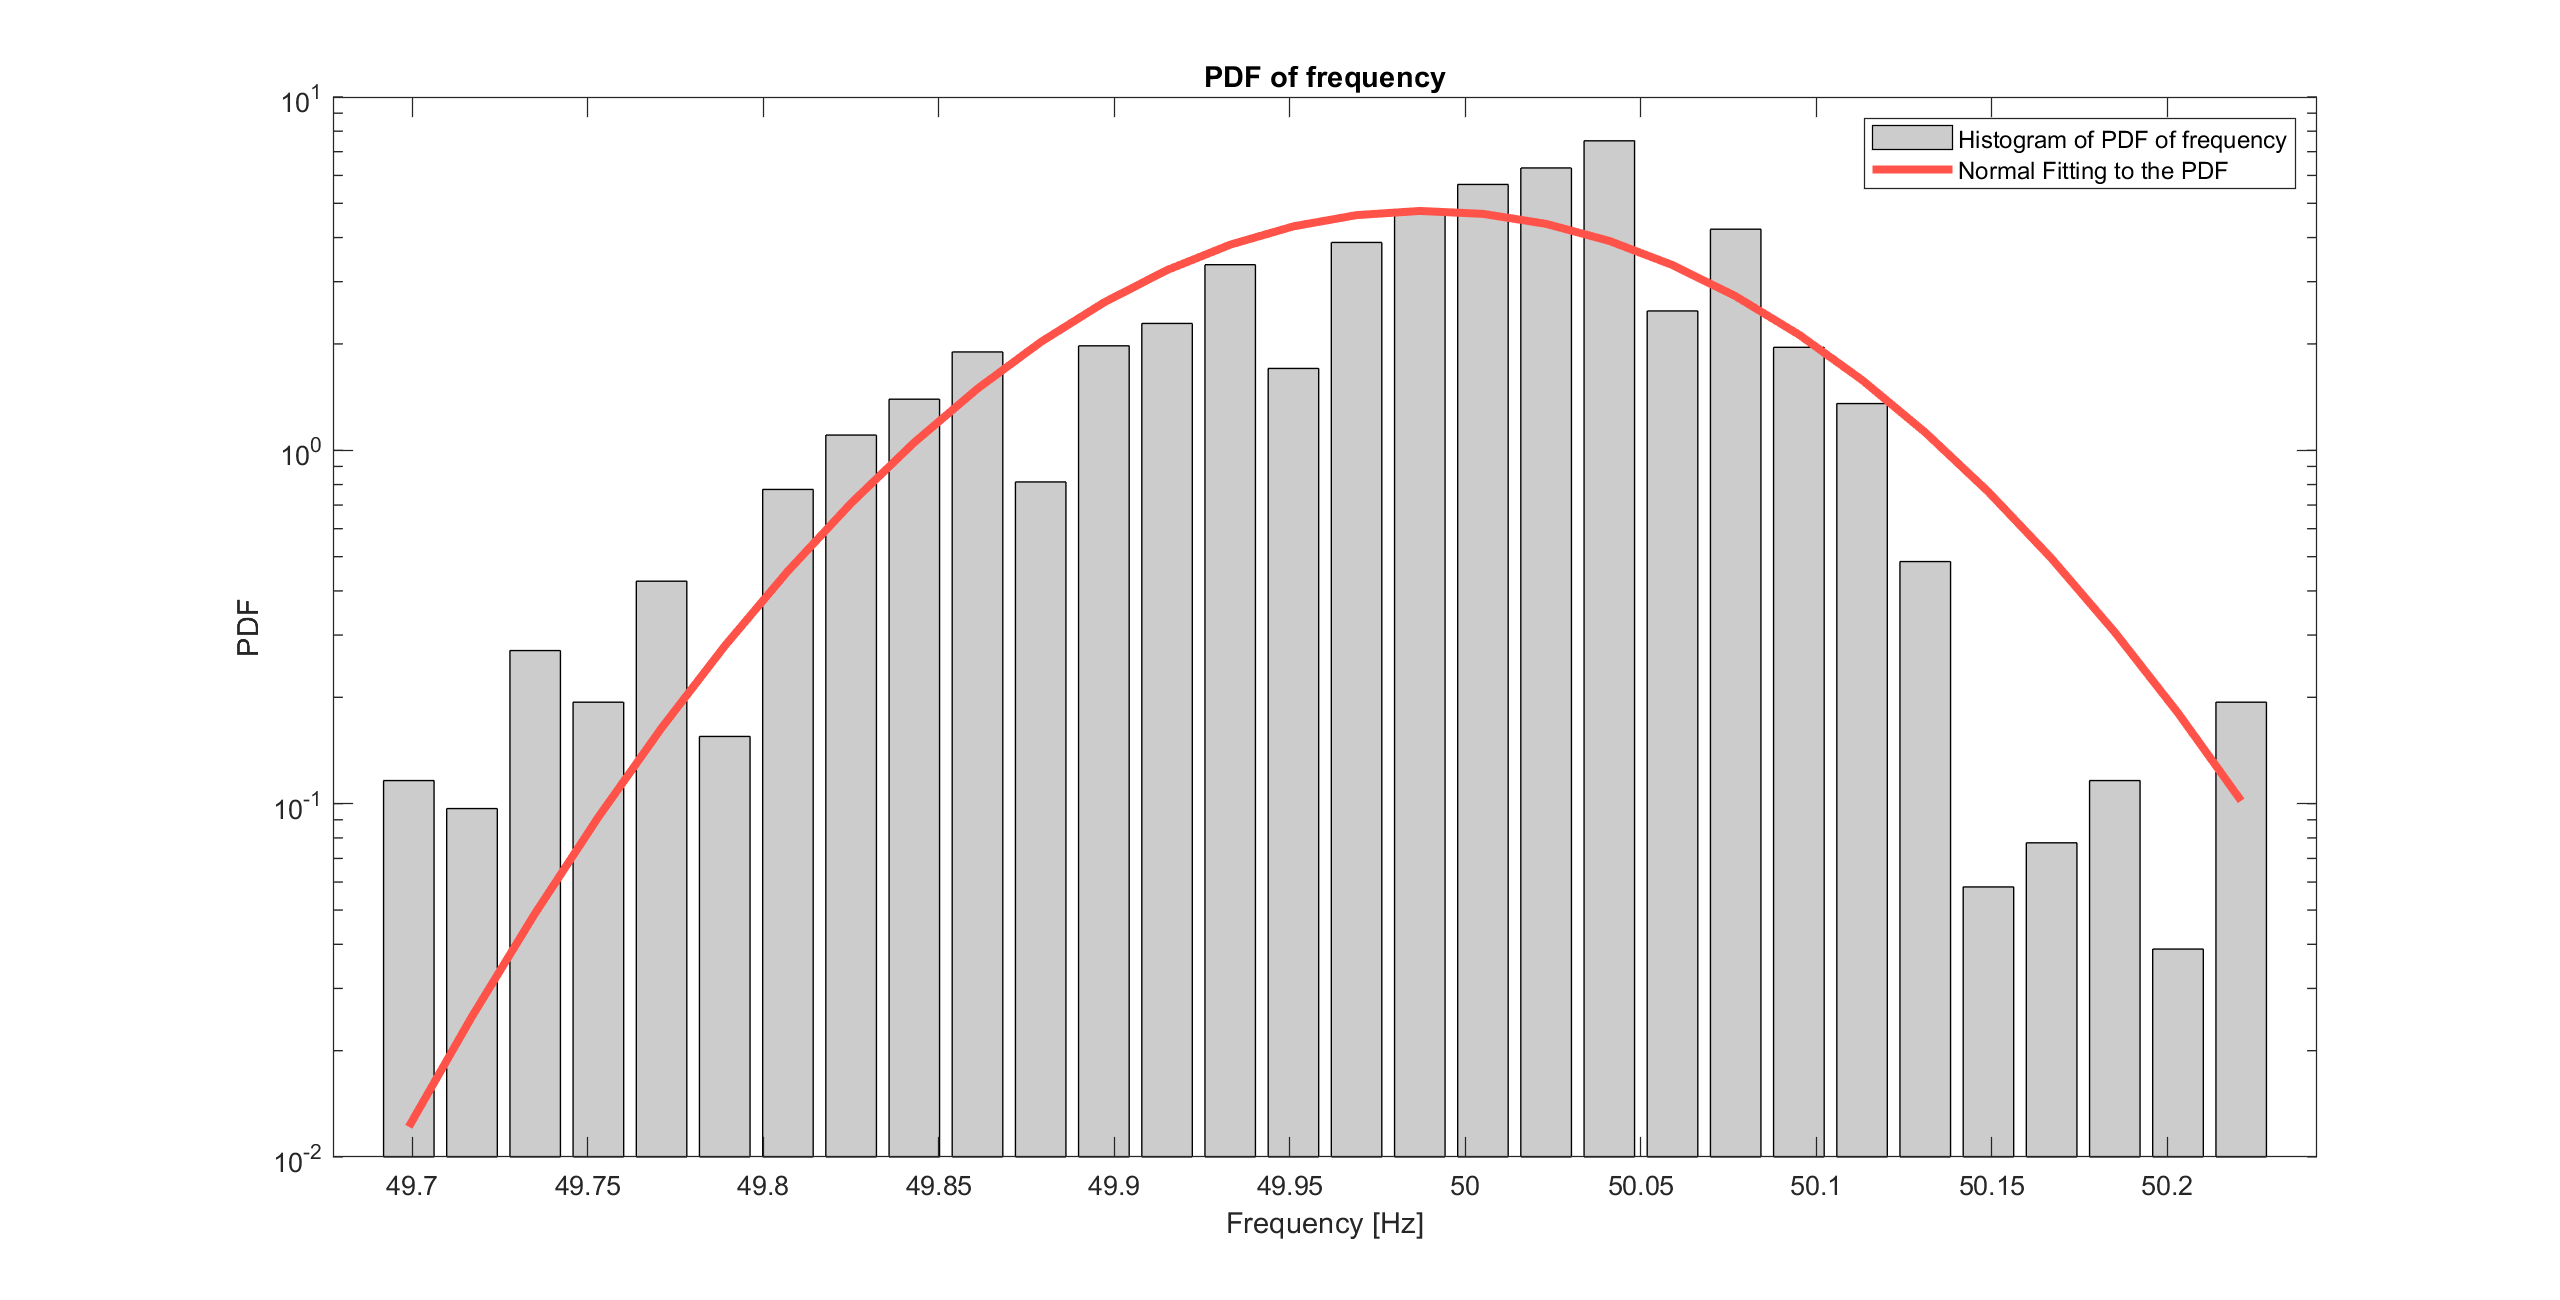
\includegraphics[width=.45\textwidth]{../figures/pdf/nrldc/pdf_frequency_nrldc_03}\quad
	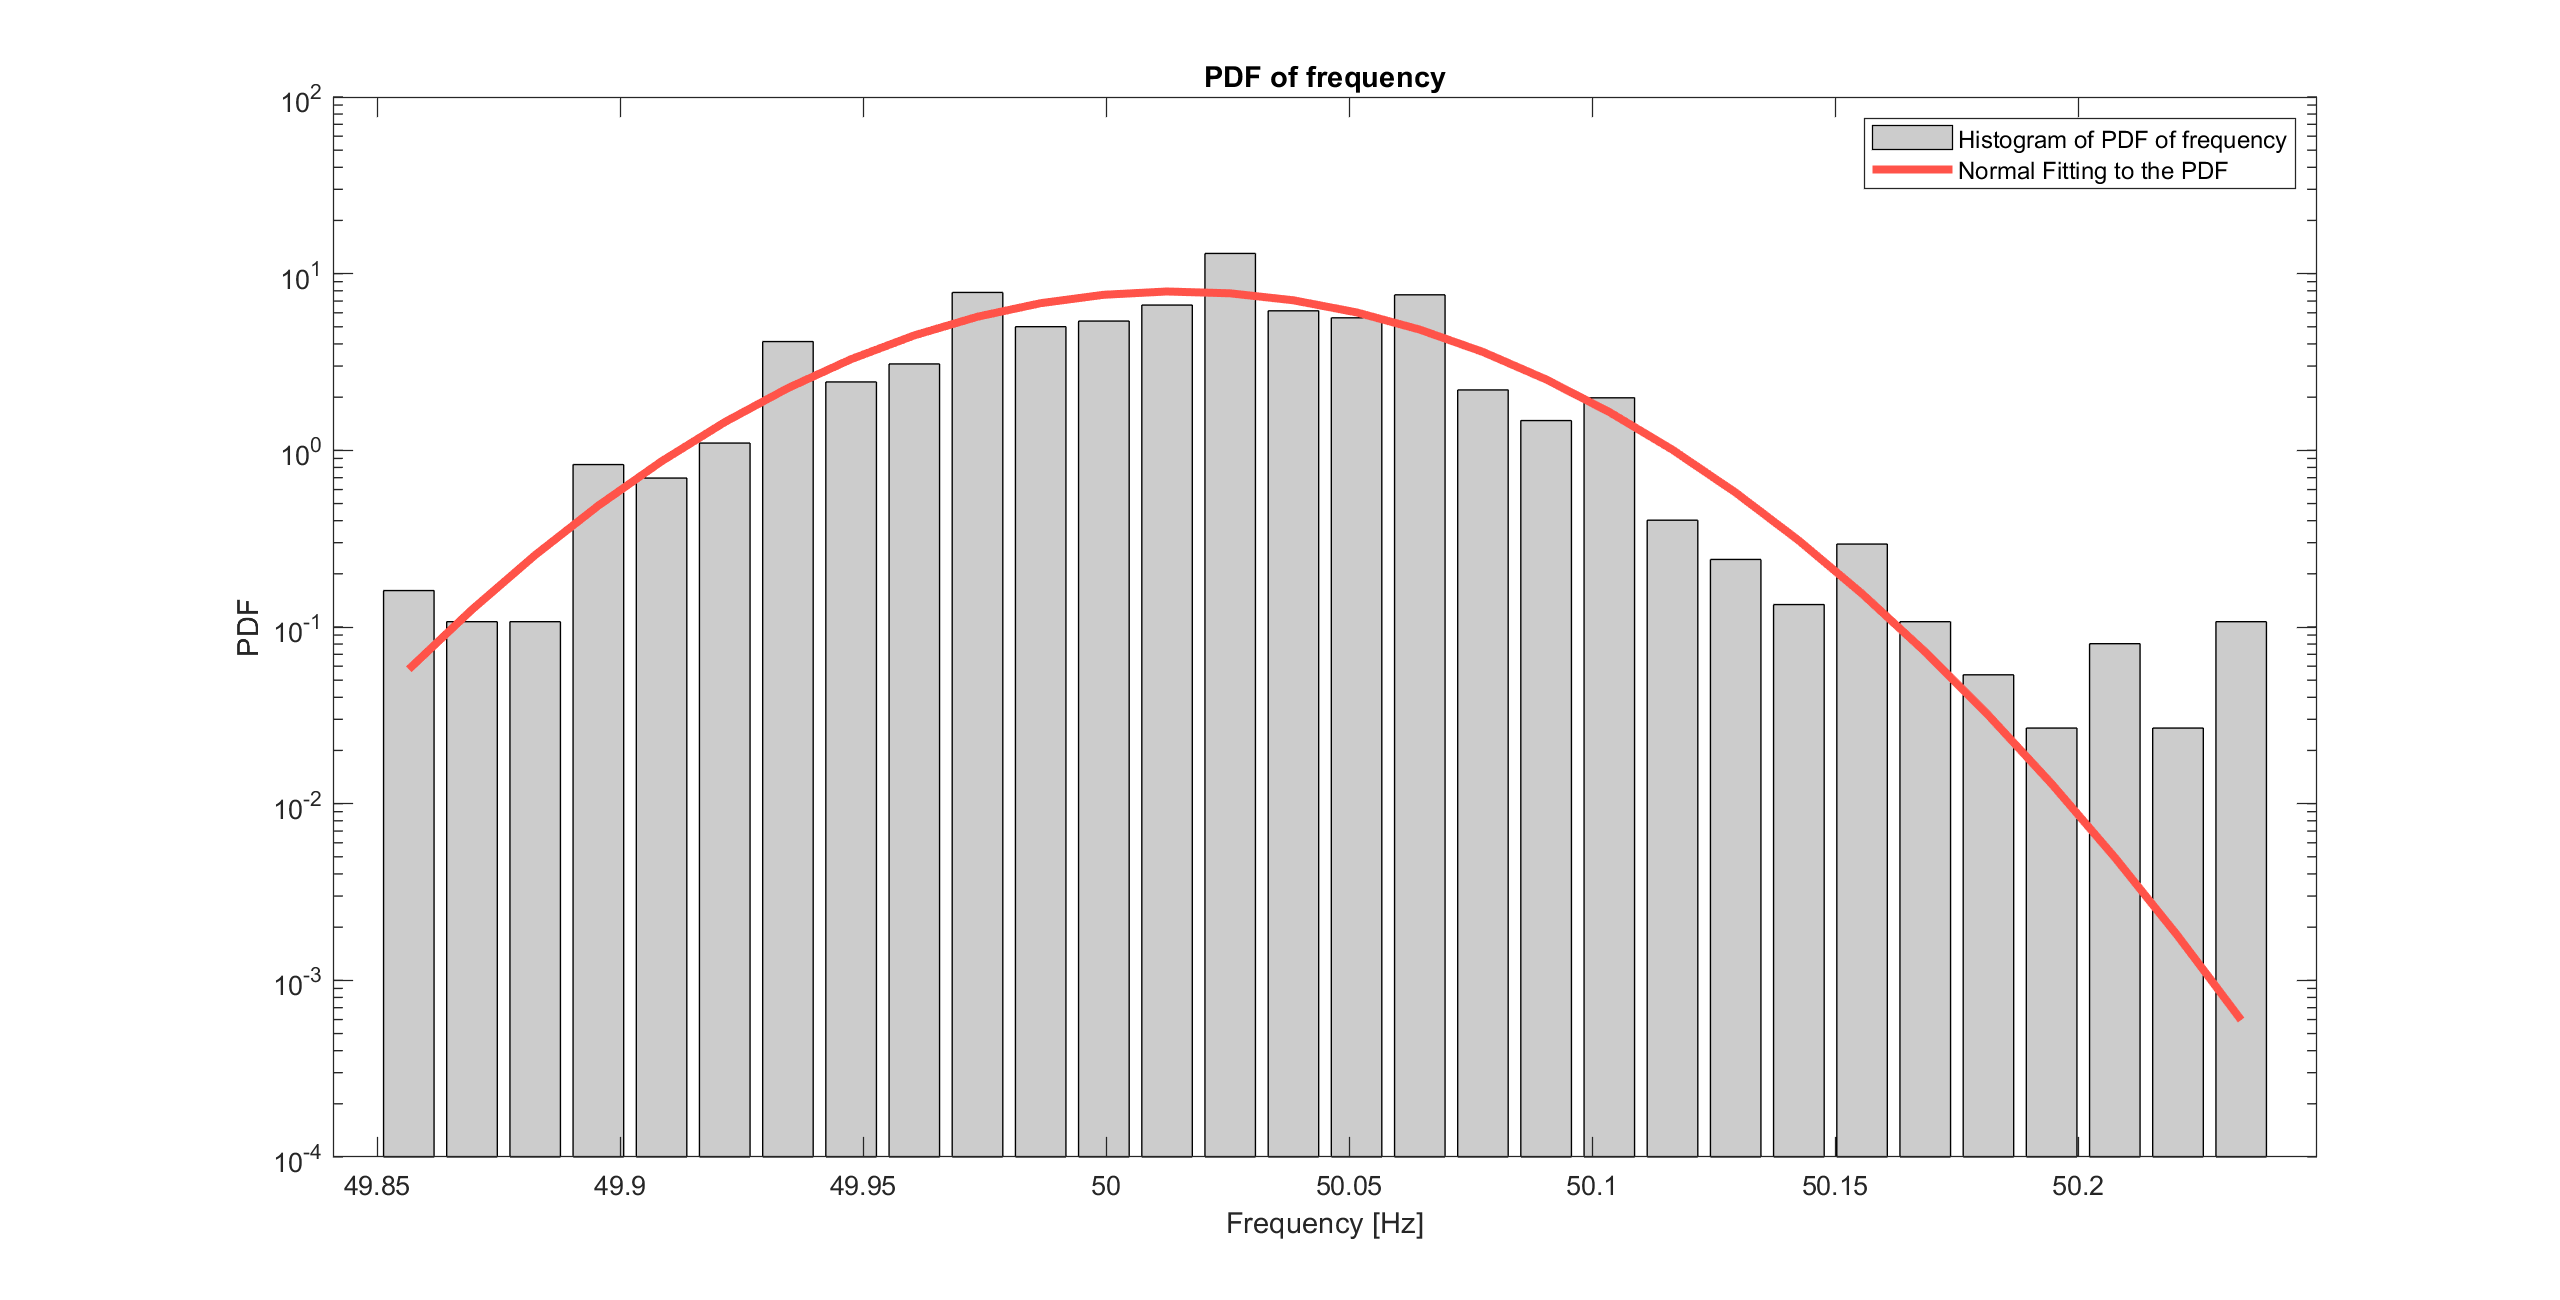
\includegraphics[width=.45\textwidth]{../figures/pdf/nrldc/pdf_frequency_nrldc_04}
	
	\medskip
	
	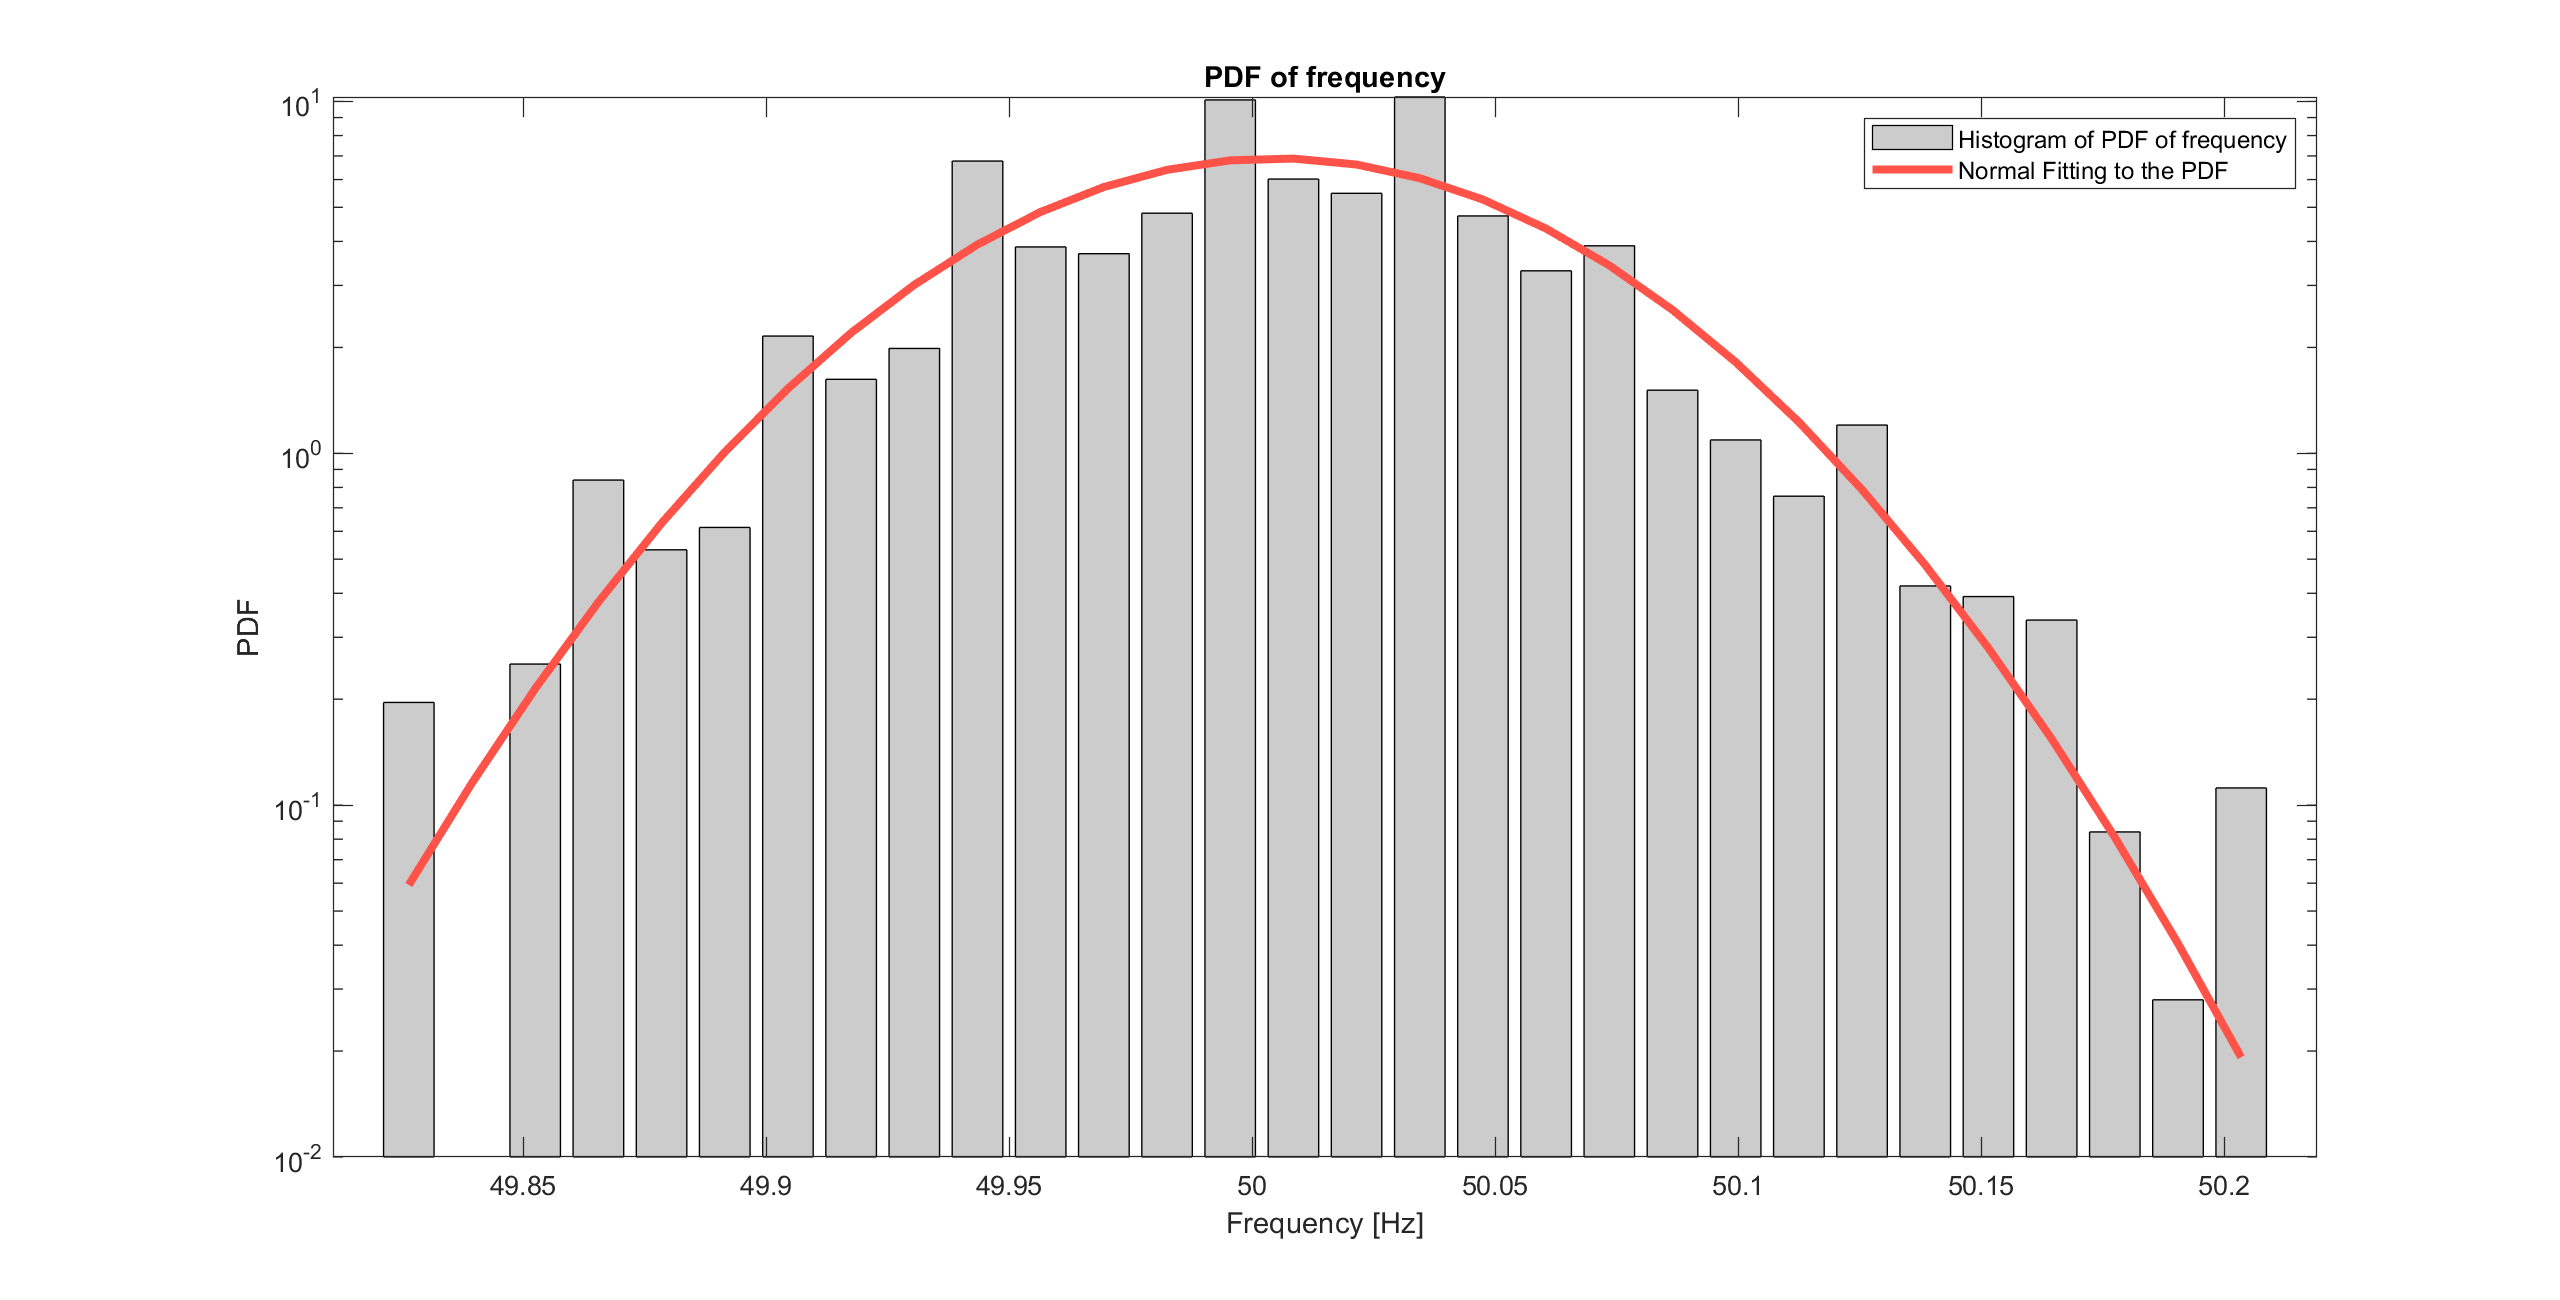
\includegraphics[width=.45\textwidth]{../figures/pdf/nrldc/pdf_frequency_nrldc_05}\quad
	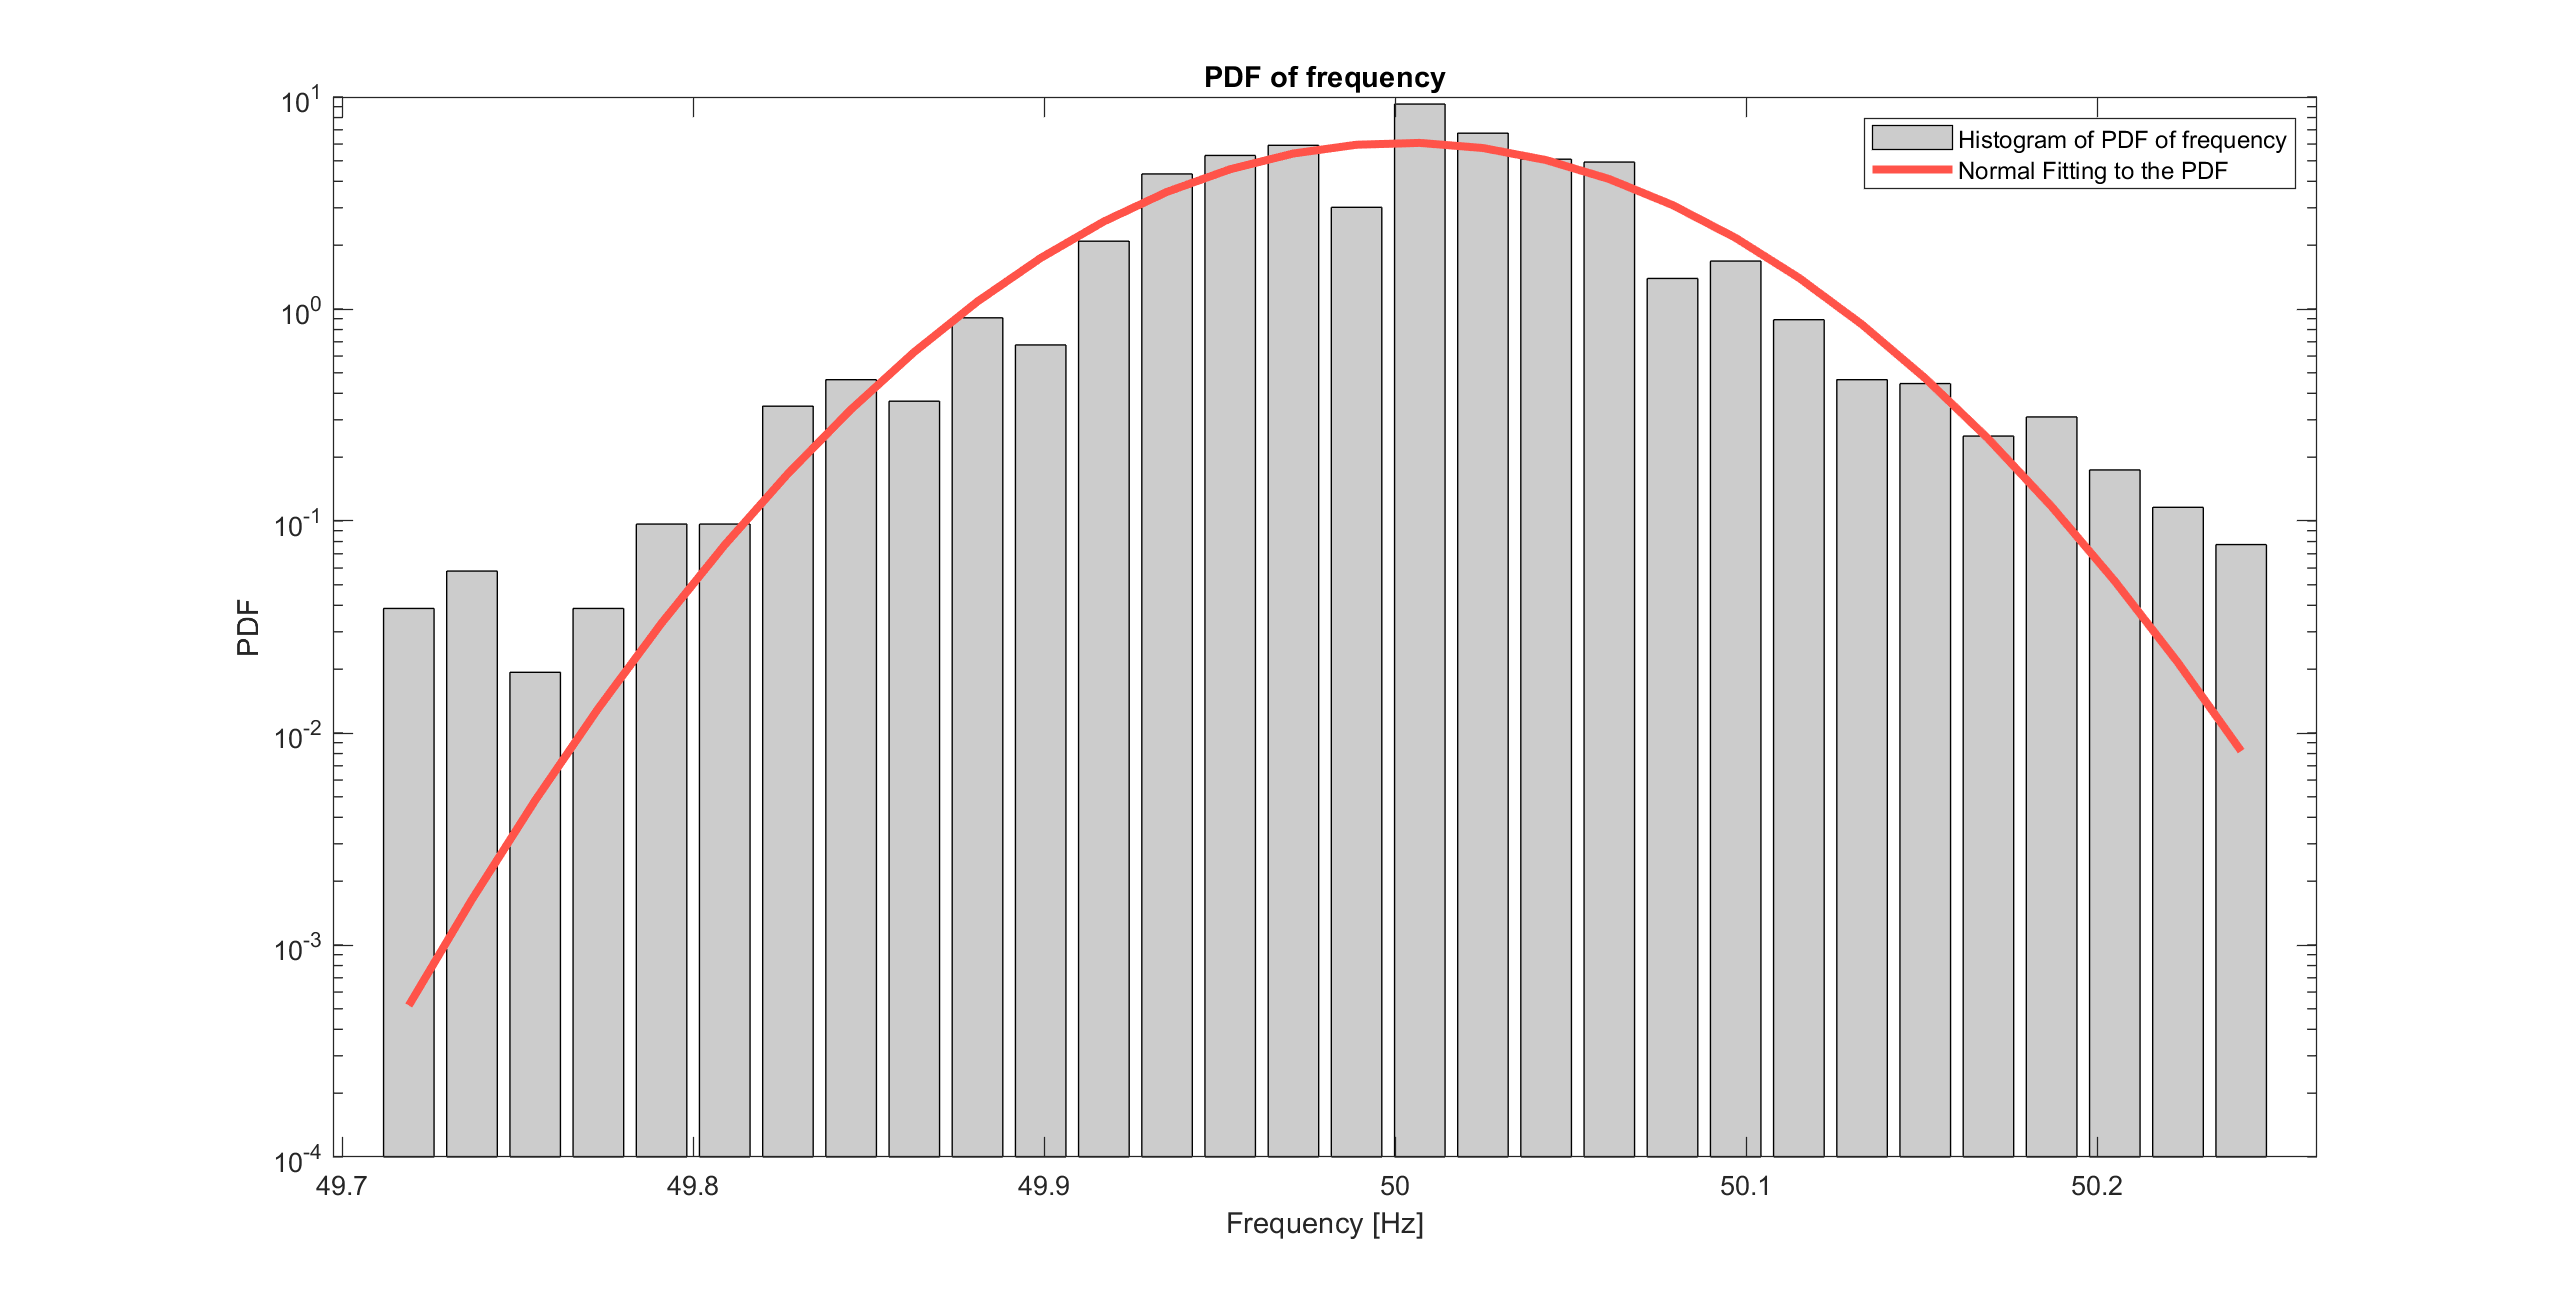
\includegraphics[width=.45\textwidth]{../figures/pdf/nrldc/pdf_frequency_nrldc_06}
	
	\caption{Frequency Probability Density Function Plots for six non-continuous days of the Indian grid (NRLDC). The frequency PDFs show considerable difference among themselves.}
\end{figure}

Thus a minimum of one month could be considered a sufficient duration to model the bulk characteristics of a grid.


